% !TeX spellcheck = sl_SI
\documentclass[11pt,a4paper,openany]{book}
\usepackage[slovene]{babel}
\usepackage[utf8]{inputenc}
\usepackage[T1]{fontenc}
\usepackage{amsmath, fullpage}
\usepackage{lmodern}
\usepackage{epsfig}
\usepackage{setspace}
\usepackage{color}
\usepackage{amsfonts}
\usepackage{url}
\usepackage{fancyhdr}
\usepackage{parskip}
\usepackage{wrapfig}
\usepackage{footnote}
% \usepackage[dvips]{graphicx}
\usepackage[titletoc]{appendix}
\usepackage[dvips]{xy}
\usepackage[font=small,format=plain,labelfont=bf,up,textfont=it,up]{caption}
\usepackage{soul}
\onehalfspacing
\makesavenoteenv{tabular}
\makesavenoteenv{table}
\usepackage[]{algorithm2e}
\usepackage{pict2e}
\usepackage[decimalsymbol=comma]{siunitx}

\begin{document}
%Velikost strani - dvostransko
\oddsidemargin 1.2cm
\evensidemargin -1.0cm
\headheight 0.5cm
\headsep 0.5cm

%Nastavitev glave in repa strani
\pagestyle{fancy}
\fancyhead{}
\renewcommand{\chaptermark}[1]{\markboth{\textsf{Poglavje \thechapter:\ #1}}{}}
\renewcommand{\sectionmark}[1]{\markright{\textsf{\thesection\  #1}}{}}
\fancyhead[RE]{\leftmark}
\fancyhead[LO]{\rightmark}
\fancyhead[LE,RO]{\thepage}
\fancyfoot{}
\renewcommand{\headrulewidth}{0.0pt}
\renewcommand{\footrulewidth}{0.0pt}

\setlength{\parindent}{0cm}

% define operators
\newcommand{\comment}[1] {
  \noindent\colorbox{yellow}{#1} \\
}

\newcommand{\mat}[1] {
  \mathsf{#1}
}


% -----------------------------------------------------------------------------
% UVODNESTRANI
% -----------------------------------------------------------------------------
% stran 1 med uvodnimi listi
\thispagestyle{empty} 

\begin{center}
{\large 
Univerza v Ljubljani\\
Fakulteta za matematiko in fiziko\\
Oddelek za fiziko
}

\vspace{3cm}
{\LARGE Klemen Kenda}\\

\vspace{2cm}
\textsc{\textbf{
\LARGE 
Uporaba metod strojnega učenja pri analizi podatkov, zajetih z ATLAS detektorjem }}

\vspace{2cm}
{ DIPLOMSKO DELO}\\
{ NA UNIVERZITETNEM ŠTUDIJU\\}

\vspace{2cm} 
{\Large Mentor: prof. dr. Tomaž Podobnik} \\
{\Large Somentor: dr. Andrej Gorišek}

\vfill
{\Large Ljubljana, 2016}
\end{center}

\newpage

%stran 2 med uvodnimi listi (prazna)
\ \thispagestyle{empty}
\newpage

% stran 3 med uvodnimi listi
\thispagestyle{empty}

\vspace{1cm}
\begin{center} 
{\Large \textbf{IZJAVA O AVTORSTVU}}
\end{center}

\begin{center} 
{\Large diplomskega dela}
\end{center}

\vspace{1cm}
Spodaj podpisani \hspace{0.5cm} Klemen Kenda,

\vspace{0.5cm}
z vpisno številko \hspace{0.65cm} 28009872,

\vspace{1cm}
sem avtor diplomskega dela z naslovom:
   
\vspace{0.5cm}
Uporaba metod strojnega učenja pri analizi podatkov, zajetih z ATLAS detektorjem

\vspace{1.5cm}
S svojim podpisom zagotavljam, da:
\begin{itemize}
	\item sem diplomsko delo izdelal samostojno pod mentorstvom 
	
	prof. dr. Tomaža Podobnika
	
	in somentorstvom 
	
	dr. Andreja Goriška
	
\end{itemize}

\vspace{1cm}
V Ljubljani, dne 15. junija 2016 \hspace{2cm} Podpis avtorja:
\newpage

%stran 4 med uvodnimi listi (prazna)
\ \thispagestyle{empty}
\newpage

% stran 5 med uvodnimi listi
\thispagestyle{empty}

$\;$ 

\vspace{5cm}
\hfill {\Large \em Morebitno posvetilo}
\thispagestyle{empty}

\vfill
Zahvala
\newpage

%stran 6 in 7 med uvodnimi listi
\newpage

\renewcommand\thepage{} 
\tableofcontents 
\renewcommand\thepage{\arabic{page}}
\thispagestyle{empty}


\newpage

\setcounter{page}{1}
\pagenumbering{arabic}


%stran 8 med uvodnimi listi (prazna)
\ \thispagestyle{empty}
\newpage



% -----------------------------------------------------------------------------
% UVOD
% -----------------------------------------------------------------------------
\chapter*{Uvod}
\addcontentsline{toc}{chapter}{Uvod}

Eksperimenta ATLAS in CMS sta leta 2012 objavila odkritje Higgsovega bozona \cite{Aad20121,Chatrchyan201230}. Eksperimenti so potekali (in še vedno potekajo) na Velikem hadronskem trkalniku (\textit{Large Hadron Collider}, LHC) v CERN-u (Evropski organizaciji za jedrske raziskave) v Ženevi \cite{ChallengeDoc}. Odkritju je leta 2013 sledila Nobelova nagrada za fiziko, ki sta jo prejela François Englert in Peter Higgs. Obstoj delca, katerega vloga je, da daje maso ostalim elementarnim delcem, je bil predviden pred skoraj petdesetimi leti. 

Higgsov bozon razpade na različne načine, ki jih v fiziki osnovnih delcev imenujemo kanali. Pri tem nastanejo novi delci. Higgsov bozon so najprej opazili v razpadnih kanalih $H \rightarrow \gamma\gamma$, $H \rightarrow Z^0Z^0$ in $H \rightarrow W^+W^-$. V naslednjem koraku je bilo potrebno najti dokaze o razpadu Higgsovega bozona v fermionske pare, v leptone $\tau$ in kvarke $b$. Dokazi o razpadih $H \rightarrow \tau^+\tau^-$ so bili predstavljeni v \cite{atlas2013,atlas2015htautau}.

Pri analizi eksperimentalnih podatkov je potrebno določiti relevantno območje faznega prostora izmerjenih značilk, v katerem je velika verjetnost, da smo naleteli na dogodke, ki nas zanimajo (v našem primeru na razpad $H \rightarrow \tau^+\tau^-$). V preteklosti so ta področja določali eksperti \textit{ročno} \cite{Adam-Bourdarios14}. Napredne klasifikacijske metode, ki temeljijo na strojnem učenju, pa se danes rutinirano uporabljajo za reševanje tega in podobnih problemov \cite{atlas2013}.

Področje dela tesno povezuje fiziko z računalništvom, natančneje s strojnim učenjem. Namen diplomskega dela je predvsem seznaniti se z uporabo metod strojnega učenja pri ločevanju signala in ozadja pri razpadu $H \rightarrow \tau^+\tau^-$, preveriti in ovrednotiti različne klasifikacijske metode na podatkih simulatorja ATLAS in preveriti proces optimizacije teh metod, ki izhaja iz podatkov (in ne nujno domenskega znanja fizike osnovnih delcev). Sekundarni cilj je razvoj lastne klasifikacijske metode, ki bo temeljila na metodi podpornih vektorjev (SVM).

\section*{Izziv HiggsML}
Z namenom, da bi izboljšali uporabljene klasifikacijske metode za reševanje prej omenjenega problema ločevanja signala od ozadja, so sodelavci kolaboracije ATLAS pripravili mednarodno tekmovanje \textit{Higgs Boson Machine Learning Challenge} (ali krajše \textit{Izziv HiggsML}) \cite{HiggsMLChallenge}, s katerim so k sodelovanju privabili zajetno množico strokovnjakov s področja strojnega učenja. Na izzivu je sodelovalo 1942 oseb, ki so skupaj pripravile 35772 rešitev. Rezultate neoptimizirane metode iz knjižnice TMVA, ki so jo je razvili in prvotno uporabljali v CERN-u, so izzivalci premagali že prvi dan izziva, kar 781 rešitev pa je bilo boljših tudi od najbolje optimizirane metode TMVA \cite{Adam-Bourdarios14}.

Pri pripravi diplomskega dela sem si pomagal s podatki, ki so bili pripravljeni posebej za omenjeni izziv, hkrati pa sem za primerjavo lastne metode in namige za izboljšavo uporabil javno dostopne rešitve, forume in druge vire v okivru izziva.

Izziv je bil namenjen širokemu naboru predvsem strokovnjakov s področja strojnega učenja, zato so sodelavci ATLAS-a surove podatke meritev že obogatili z večino relevantnimi izpeljankami, ki izhajajo iz domenskega znanja fizike visokih energij. Ob tem se je izkazalo, da nadaljnje poglabljanje v izpeljavo fizikalno relevantnih značilk načeloma ni prineslo znatnega izboljšanja končnih rezultatov\footnote{\url{https://www.kaggle.com/c/higgs-boson/forums/t/10350/how-physicists-fared}}.


\section*{Terminologija}
\addcontentsline{toc}{section}{Terminologija}

Ker je področje strojnega učenja in umetne inteligence v slovenskem prostoru majhno in ker se slovenska terminologija na tem področju še redkeje uporablja in je zato tudi strokovno podkovanemu bralcu manj znana, na tem mestu prilagam kratek slovarček strokovnih terminov s področja strojnega učenja. Vsi prevodi temeljijo na \textit{Računalniškem slovarčku}, ki ga vzdržuje Odsek za inteligentne sistem na Inštitutu "Jožef Stefan"\footnote{\url{http://dis-slovarcek.ijs.si}}. Slovarček je prikazan v tabeli \ref{slovar}.

\begin{table}[ht]
	\centering
	\begin{tabular}{ll}
		\hline
		\textbf{Slovenski izraz} & \textbf{Angleški izraz} \\
		\hline
		analiza glavnih komponent & principal component analysis, PCA \\
		grozdenje & clustering \\
		metoda podpornih vektorjev & support vector machine, SVM \\
		oznaka & label \\
		potrjevalna podatkovna množica & validation set \\
		raziskovalna analiza & exploratory analysis \\
		vektor značilk & feature vector \\
		učna podatkovna množica & training set \\		
		značilka & feature \\
	\end{tabular}
	\caption{Slovensko-angleški slovarček izrazov s področja strojnega učenja.}
	\label{slovar}
\end{table}


% -----------------------------------------------------------------------------
% POGLAVJE: Fizikalne osnove
% -----------------------------------------------------------------------------
\chapter{Fizikalne osnove}
\label{ch:basics}
Standardni model (SM) osnovnih delcev opisuje osnovne gradnike snovi in interakcije med njimi. V SM interakcije potekajo z izmenjavo bozonov s spinom 1. Bozoni se izmenjujejo med elektromagnetnimi, šibkimi in močnimi naboji. Delci polja, ki posredujejo elektromagnetno in močno interakcijo (foton in gluoni), so bozoni brez mase. Nosilci šibke interakcije, bozoni $W^+$, $W^-$ in $Z^0$, pa imajo maso približno 100-krat večjo od protona. Nosilci naboja so elementarni fermioni s spinom $\frac{1}{2}$: šest kvarkov in šest leptonov (ter pripadajočih antidelcev). Shematski prikaz SM je na sliki \ref{sl:sm}.

\begin{figure}[ht]
	\centering
	\includegraphics[width=12.0cm]{physics/sm.pdf}
	
	\caption{ Standardni model elementarnih delcev, s tremi generacijami gradnikov snovi in z bozoni s spinom 1 v četrtem stolpcu ter Higgsovim bozonom v petem \cite{WikiSM}. }
	\label{sl:sm}
\end{figure}

Teoretični fiziki so pred petimi desetletji napovedali obstoj polja, ki prežema prostor in daje energijo vakuumu. Obstoj polja je bil potreben za pojasnitev mas bozonov $W^+$, $W^-$ in $Z^0$. V primeru zadostne količine razpoložljive energije bi lahko z vzbuditvijo tega polja nastal masiven delec s spinom 0: Higgsov bozon, ki ga označujemo s $H$. Higgsov bozon je nestabilen, zato hitro razpade v druge delce \cite{AadScience2012, ChallengeDoc}. 

Standardni model ne napoveduje mase $H$. Napoveduje pa, ob določeni masi $H$, relativno pogostost (razvejitvena razmerja) posameznih razpadnih načinov Higgsovega bozona, ki je prikazana v tabeli \ref{tb:pdghiggs}. Različna razmerja eksperimentalno izmerimo in jih primerjamo z napovedmi standardnega modela, s tem pa preverimo, ali je delec, ki smo ga opazili, v resnici Higgsov bozon.

\begin{table}[ht]
	\centering
	\begin{tabular}{lr}
		\hline
		\textbf{Razpadni kanal} & \textbf{Razmejitveno razmerje} \\
		\hline
		$H \rightarrow \gamma\gamma$ & $\num{2,28} \times 10^{-3}$ \\	
		$H \rightarrow Z^0Z^0$ & $\num{2,64} \times 10^{-2}$ \\
		$H \rightarrow W^+W^-$ & $\num{2,15} \times 10^{-1}$ \\
		$H \rightarrow \tau^+\tau^-$ & $\num{6,32} \times 10^{-2}$ \\
		$H \rightarrow b\bar{b}$ & $\num{5,77} \times 10^{-1}$ \\
		$H \rightarrow Z^0\gamma$ & $\num{1,54} \times 10^{-3}$ \\
		$H \rightarrow \mu^+\mu^-$ & $\num{2,19} \times 10^{-4}$
	\end{tabular}
	\caption{Razmejitvena razmerja za Higgsov bozon z maso $m_H = 125\,\text{GeV}$ po standardnem modelu\cite{PDGHiggs}.}
	\label{tb:pdghiggs}
\end{table}

\section{Izpeljava relevantnih značilk}
Podpoglavje opisuje nekaj osnovnih enačb iz posebne teorije relativnosti, ki so potrebne za razumevanje fizikalnega ozadja problema, hkrati pa so potrebne za izpeljavo novih relevantnih značilk iz izmerjenih podatkov. V celotnem diplomskem delu uporabljam termin \textit{značilka} s področja strojnega učenja, nanaša pa se predvsem na različne izmerjene ali izpeljane fizikalne količine, ki služijo kot vhodni podatki pri reševanju problema ločevanja signala od ozadja. Večina fizikalno pomembnih značilk je bila izračunanih že v izvornih podatkih, ki sem jih uporabil v diplomi. Celoten seznam značilk, ki sem jih uporabljal, si je moč ogledati v razdelku \ref{ch:opis_podatkov}, spodnji opis pa je povzet po \cite{ChallengeDoc}.

\subsection{Gibalna količina, masa in energija}
Osnovna enačba posebne teorije relativnosti je
\begin{equation}
E^2 = p^2c^2 + m^2c^4,
\label{eq:4momentum}
\end{equation}
kjer je $E$ energija delca, $p$ njegova gibalna količina, $m$ lastna masa (masa v mirovanju) in $c$ hitrost svetlobe v praznem prostoru. V literaturi se avtorji velikokrat držijo dogovora o izpuščanju $c$ iz izrazov kot je enačba \ref{eq:4momentum}, ki s tem preide v 
\begin{equation}
E^2 = p^2 + m^2.
\label{eq:4momentumsimplified}
\end{equation}

\noindent Tega dogovora se držim tudi v svojem diplomskem delu.

Gibalna količina je povezana s hitrostjo delca $v$.  Za delec z neničelno maso v posebni teoriji relativnosti velja zveza $p = \gamma m v$, kjer je $p$ oznaka za gibalno količino, $m$ masa delca, $\gamma$ pa je definirana kot
\begin{equation}
\gamma = \frac{1}{\sqrt{1 - (v/c)^2}}.
\label{eq:gamma}
\end{equation}
Enačba velja tako za velikosti, kakor tudi za tridimenzionalne vektorje $\mathbf{v}$ in $\mathbf{p}$. Zapišemo lahko $\mathbf{p} = \gamma m \mathbf{v}$, pri tem pa velja dogovor $p = |\mathbf{p}|$ in $v = |\mathbf{v}|$. Faktor $\gamma$ ob približevanju $v$ svetlobni hitrosti $c$ divergira proti $\infty$, kar pomeni, da svetlobne hitrosti delcem z neničelno maso ni mogoče doseči ali preseči. Kinematika delca je popolnoma definirana z vektorjem gibalne količine in energijo, torej s četvercem $(p_x, p_y, p_z, E)$. Ko delec identificiramo, ima le-ta dobro definirano maso, tako da lahko energijo izračunamo s pomočjo gibalne količine z enačbo \ref{eq:4momentumsimplified}. Namesto komponent gibalne količine $p_x,\;p_y$ in $p_z$ velikokrat uporabimo parametre $\phi, \eta$ in $p_T$. $\phi$ je azimutalni kot vektorja gibalne količine (v prečni ravnini). $\eta$ je psevdorapidnost, ki je definirana z
\begin{equation}
\eta = -\ln \tan(\theta/2),
\label{eq:pseudorapidity}
\end{equation}
pri čemer je $\theta$ polarni kot vektorja gibalne količine (z osjo $z$). $p_T$ predstavlja prečno gibalno količino delca in je definiran z enačbo
\begin{equation}
p_T = \sqrt{p_x^2 + p_y^2}.
\label{eq:transversemomentum}
\end{equation}
Zadnje tri količine so natančneje opisane v razdelku \ref{sec:atlasdetector}.

\subsection{Invariantna masa in manjkajoča prečna energija}
Masa delca je njegova notranja lastnost. Za vse dogodke, povezane s Higgsovim bozonom pričakujemo, da bodo imeli enako maso. Da bi maso Higgsovega bozona lahko izmerili, potrebujemo četverce $(p_x, p_y, p_z, E) = (\mathbf{p}, E)$ vseh razpadnih produktov. Denimo, da Higgsov bozon razpade v $N$ delcev, katerih četverce izmerimo s pomočjo detektorja. S pomočjo ohranitvenih zakonov za energijo in gibalno količino tako lahko zapišemo $E_H = E_1 + E_2 + E_3 + ... + E_N$ in $\mathbf{p}_H = \mathbf{p}_1 + \mathbf{p}_2 + \mathbf{p}_3 + ... + \mathbf{p}_N$. Invariantno maso kandidata za Higgsov bozon pa lahko izračunamo iz enačbe \ref{eq:4momentumsimplified}.

Pri topologiji razpada $H \rightarrow \tau^+\tau^-$, ki je predmet diplomske naloge (glej naslednje podpoglavje), končno stanje sestavljajo lepton, hadronski tau in trije nevtrini. Lastnosti leptona in hadronskega tau izmerimo s pomočjo detektorja, od nevtrinov pa poznamo samo manjkajočo prečno energijo ($\mathbf{E^{miss}_T}$), ki predstavlja oceno vsote gibalnih količin treh nevtrinov v prečni ravnini. Mase $H$ torej ne moremo izmeriti, zato se moramo zanesti na oceno s pomočjo količin, ki so povezane z maso primarnih produktov razpada ($\tau^+\tau^-$).

\subsection{Druge uporabne formule in dogovori}

V diplomskem delu bom uporabljal konvencionalni referenčni okvir detektorja ATLAS (glej sliko \ref{detektoratlasokvir}). Os $z$ kaže vzdolž horizontalne linije žarka, osi $x$ in $y$ razpenjata na žarek pravokotno ravnino, pri čemer je os $y$ usmerjena proti vrhu detektorja. $\theta$ je polarni kot, $\phi$ pa azimutalni kot. Prečne količine so tiste, ki jih projiciramo na ravnino $x\text{-}y$, torej tiste količine, kjer je koordinata $z$ izpuščena. 

\begin{figure}[h!]
	\centering
	\setlength{\unitlength}{1cm}
	\begin{picture}(10,5)
	% arrows
	\put(5, 2.5){\vector(-1, -1){2}}
	\put(5, 2.5){\vector(0, 1){2.5}}
	\put(5, 2.5){\vector(1, 0){4}}
	
	% labels
	\put(3.4, 0.5){\makebox(0, 0){$x$}}
	\put(5.3, 4.7){\makebox(0, 0){$y$}}
	\put(9, 2){\makebox(0, 0){$z$}}
	
	%cylinder
	\color{blue}
	\put(0.9, 1){	\line(1, 0){8} }
	\put(0.9, 4){	\line(1, 0){8} }
	\qbezier(1, 1)(0.6, 1)(0.5, 2.5)
	\qbezier(1, 1)(1.4, 1)(1.5, 2.5)
	\qbezier(1, 4)(0.6, 4)(0.5, 2.5)
	\qbezier(1, 4)(1.4, 4)(1.5, 2.5)
	
	\qbezier(9, 1)(8.6, 1)(8.5, 2.5)
	\qbezier(9, 1)(9.4, 1)(9.5, 2.5)
	\qbezier(9, 4)(8.6, 4)(8.5, 2.5)
	\qbezier(9, 4)(9.4, 4)(9.5, 2.5)
	
	\color{red}
	\put(5, 2.5){\line(3,1){3}}
	\qbezier(7, 2.5)(7, 2.8)(6.85,3.12)
	\put(7.2, 2.8){\makebox(0,0){$\theta$}}
	\color{green}
	\put(5, 2.5){\line(-1,3){0.33} }
	\put(4.53,3.5) { \line(1, 0){3.33} }
	\qbezier(4.7, 2.2)(4.6, 2.65)(4.8,3.1)
	\put(4.35,2.65){\makebox(0,0){$\phi$}}
	
	\end{picture}
	\caption{Referenčni okvir detektorja ATLAS \cite{ChallengeDoc}.}
	\label{detektoratlasokvir}
\end{figure}

\noindent Vektor gibalne količine lahko zapišemo s pomočjo predhodno razloženih količin $p_T, \phi$ in $\eta$ kot
\begin{eqnarray}
\mathbf{p} = \left( 
\begin{array}{c}
p_x \\
p_y \\
p_z 
\end{array}
\right) = \left(
\begin{array}{c}
p_T \cos \phi \\
p_T \sin \phi \\
p_T \sinh \eta
\end{array}
\right).
\label{eq:momentum}
\end{eqnarray}
Modulus $p$ je definiran kot
\begin{eqnarray}
p_T \cosh \eta.
\label{eq:modulus}
\end{eqnarray}
Manjkajoča prečna energija $\mathbf{E}^{miss}_T$ je dvodimenzionalni vektor
\begin{eqnarray}
\mathbf{E}^{miss}_T = \left(
\begin{array}{c}
|\mathbf{E}^{miss}_T| \cos \phi_T \\
|\mathbf{E}^{miss}_T| \sin \phi_T \\
\end{array}
\right),
\label{eq:emisst}
\end{eqnarray}
kjer je $\phi_T$ azimutalni kot manjkajoče prečne energije.

Invarianta masa dveh delcev z definiranima četvercema gibalne količine je
\begin{eqnarray}
m_{inv}(\mathbf{a}, \mathbf{b}) =
\sqrt{
	\left(
	\sqrt{a_x^2 + a_y^2 + a_z^2} + \sqrt{b_x^2 + b_y^2 + b_z^2}
	\right)^2
	- (a_x + b_x)^2
	- (a_y + b_y)^2
	- (a_z + b_z)^2
}.
\label{eq:invmass}
\end{eqnarray}
Prečna masa dveh delcev je enaka invariantni masi vektorske vsote, pri čemer komponenti v $z$ smeri postavimo na 0:
\begin{eqnarray}
m_{tr}(\mathbf{a}, \mathbf{b}) =
\sqrt{
	\left(
	\sqrt{a_x^2 + a_y^2} + \sqrt{b_x^2 + b_y^2}
	\right)^2
	- (a_x + b_x)^2
	- (a_y + b_y)^2
}.	
\label{eq:invmasstransverse}
\end{eqnarray}
Psevdorapidnostno ločitev med delcema $A$ in $B$ definiramo kot
\begin{eqnarray}
|\eta_A - \eta_B|.
\label{eq:pseudorapidityseparation}
\end{eqnarray}
$R$-ločitev med delcema $A$ in $B$ zapišemo kot
\begin{eqnarray}
\sqrt{(\eta_A - \eta_B)^2 + (\phi_A - \phi_B)^2},
\label{eq:rseparation}
\end{eqnarray}
pri čemer $\phi_A - \phi_B$ pretvorimo nazaj na interval $[-\pi, \pi]$. 

\section{Razpad $H \rightarrow \tau^+\tau^-$}

Higgsov bozon z maso $125\,\text{GeV}$ lahko razpade na različne načine, ki so prikazani v tabeli \ref{tb:pdghiggs}. V letih 2011 in 2012 so se pri eksperimentu ATLAS osredotočili na dva najbolj karakteristična kanala: $H \rightarrow \gamma\gamma$ in $H \rightarrow ZZ \rightarrow \ell\ell\ell\ell$. 

\textbf{Kanal} ${\mathbf H \rightarrow \gamma\gamma}$. Higgsov bozon na dva fotona razpade samo v $\num{0,228}\%$ primerih. Kljub nizkemu razmejitvenemu razmerju pa je prednost tega razpada, da imata fotona z visoko energijo v detektorju precej jasno signaturo in je tako identifikacija takega dogodka relativno preprosta \cite{AadScience2012}.

Zanima nas vsota energij obeh fotonov, ki izhaja iz mase delca, iz katerega sta nastala. Detektor ATLAS izmeri kota $\phi$ in $\theta$ obeh fotonov ter njuni energiji. S pomočjo enačb \ref{eq:4momentumsimplified}, \ref{eq:pseudorapidity}, \ref{eq:momentum} lahko izračunamo vse potrebne količine za izračun invariantne mase kandidata za Higgsov bozon, kar storimo s pomočjo enačbe \ref{eq:invmass}.

Masni spekter dogodkov $\gamma\gamma$ je predstavljen na sliki \ref{sl:hgammagamma}. Spekter opisujeta vsoti gladkega parametričnega modela ozadja in modela signala, ki ima obliko gaussove krivulje s podaljšanima repoma. Na sliki je viden majhen, vendar statistično signifikanten vrh pri $m_{\gamma\gamma} = \num{126,5}\,\text{GeV}$. Spodnji del slike prikazuje odstopanje podatkov glede na model ozadja.

\begin{figure}[ht]
	\centering
	\includegraphics[width=8.0cm]{physics/hgammagammamass.pdf}
	
	\caption{ Masni spekter dogodkov $\gamma\gamma$ \cite{AadScience2012}. }
	\label{sl:hgammagamma}
\end{figure}


\textbf{Kanal} $\mathbf{H \rightarrow ZZ \rightarrow \ell\ell\ell\ell}$. V tem razpadnem načinu Higgsov bozon razpade na dva bozona $Z$, vsak od njiju pa naprej v par leptonov ($e^+e^-$ ali $\mu^+\mu^-$). Ker samo $7\%$ bozonov $Z$ razpade na tak način, je pričakovano število dogodkov zelo nizko (v prvem eksperimentu so pričakovali samo 6 dogodkov za maso $m_H = 126\,\text{GeV}$) \cite{AadScience2012}. Rezultati so prikazani na sliki \ref{sl:hzz}.

\begin{figure}[ht]
	\centering
	\includegraphics[width=8.0cm]{physics/hzz.pdf}
	
	\caption{ Masni spekter dogodkov $\ell\ell\ell\ell$ \cite{AadScience2012}. }
	\label{sl:hzz}
\end{figure}

Manjši vrh pri $90\,\text{GeV}$ predstavlja en bozon $Z$, ki razpade na 4 leptone. Širši vrh pri $200\,\text{GeV}$ pa predstavlja neposredni nastanek parov bozonov $Z$. Dodaten vrh je v okolici $125\,\text{GeV}$ in sovpada s pričakovanim signalom, ki je na sliki prikazan s svetlo modro barvo.


\textbf{Kanal} ${\mathbf H \rightarrow \tau^+\tau^-}$. Razpadni način $H \rightarrow \tau^+\tau^-$ je predmet obravnave poenostavljenega problema razločevanja signala od ozadja v izzivu \textit{HiggsML}, s katerim se ukvarjam v diplomskem delu. Slika \ref{sl:htautaumass} prikazuje masna spektra podobnih razpadov $H \rightarrow \tau^+\tau^-$ in $Z \rightarrow \tau^+\tau^-$, ki sta bila izdelana s pomočjo simulatorja detektorja ATLAS. 

\begin{figure}[ht]
	\centering
	\includegraphics[width=8.0cm]{physics/htautau-mass.pdf}
	
	\caption{ Rekonstruirana invarianta masa simuliranih dogodkov $\tau\tau$ \cite{atlas2013}. }
	\label{sl:htautaumass}
\end{figure}

V primerjavi s slikama \ref{sl:hgammagamma} in \ref{sl:hzz} opazimo, da je vrh pri $m_H$ znatno širši, zaradi česar je ločevanja signala od ozadja, s tem pa je tudi določanje razvejitvenega razmerja $H \rightarrow \tau^+\tau^-$, v tem primeru težavnejše. Ker se nevtrinov v detektorju ne meri, je namreč na podlagi (nepopolnega) končnega stanja težko ovrednotiti končno maso kandidata za Higgsov bozon. Prav tako lahko tudi bozon $Z$ razpade v dva delca $\tau$, pri čemer je verjetnost za takšen dogodek v detektorju ATLAS precej večja od verjetnosti za razpad iz $H$. Ker je masa $Z$ ($91\,\text{GeV}$) v bližini mase $H$ ($125\,\text{GeV}$), sta si razpada glede končnih produktov zelo podobna in ju je zato težko razločiti \cite{ChallengeDoc}.

Delec $\tau$ je nestabilen. Njegova povprečna življenska doba je $2,9 \times 10^{-13}\,\text{s}$ \cite{WikiTau}. Nekaj najbolj verjetnih razpadnih kanalov in razvejitvenih razmerij je prikazanih v tabeli \ref{tb:pdgtau}.

\begin{table}[ht]
	\centering
	\begin{tabular}{lr}
		\hline
		\textbf{Razpadni kanal} & \textbf{Razmejitveno razmerje} \\
		\hline
		$\tau \rightarrow \pi^-\pi^0\nu_\tau$ & $\num{2,551} \times 10^{-1}$ \\	
		$\tau \rightarrow e^-\bar{\nu}_e\nu_\tau$ & $\num{1,785} \times 10^{-1}$ \\
		$\tau \rightarrow \mu^-\bar{\nu}_\mu\nu_\tau$ & $\num{1,736} \times 10^{-1}$ \\
		$\tau \rightarrow \pi^-\nu_\tau$ & $\num{1,091} \times 10^{-1}$ \\
		$\tau \rightarrow \pi^-\pi^+\pi^-\nu_\tau$ & $\num{9,00} \times 10^{-2}$ \\
		$\tau \rightarrow \pi^-\pi^+\pi^-\pi^0\nu_\tau$ & $\num{2,70} \times 10^{-2}$ \\	\end{tabular}
	\caption{Razmejitvena razmerja najpogostejših razpadnih načinov delca $\tau$ \cite{PDGTau}.}
	\label{tb:pdgtau}
\end{table}

V diplomskem delu sem obravnaval eno izmed topologij razpada, in sicer dogodke, kjer en delec $\tau$ razpade v elektron ali mion ter dva nevtrina, drugi $\tau$ pa v hadrone in en nevtrino.

\begin{figure}[h]
	\includegraphics[width=16.0cm]{physics/htautau.pdf}
	
	\caption{Primer dogodka $H \rightarrow \tau^+\tau^-$, kjer delca $\tau$ razpadeta na mion in elektron. Elektron je prikazan z modro sledjo, mion pa z rdečo. Približno vodoravna črtkana črta v ravnini $R-\phi$ prikazuje smer vektorja $\mathbf{E_T^{miss}}$, na sliki sta še dva VBF (\textit{vector boson fusion}) pljuska, označena s turkiznima stožcema \cite{atlas2015htautau}.  }
	\label{htautau}
\end{figure}

Slika \ref{htautau} prikazuje primer dogodka $H \rightarrow \tau^+\tau^-$. Rezultati projekta ATLAS so bili prvič predstavljeni leta 2013 v \cite{atlas2013}, uradno pa leta 2015 v \cite{atlas2015htautau}. Pri analizi so avtorji uporabili poln nabor trkov protonov, ki jih je eksperiment ATLAS posnel na LHC med leti 2011 in 2012. Za ločitev dogodkov od ozadja so uporabili algoritem, ki je temeljil na pospešenem gradientnem spustu nad ansambli odločitvenih dreves. Uporabili so vse kombinacije leptonskih in hadronskih razpadov tau.

\section{Detektor ATLAS}
\label{sec:atlasdetector}
Veliki hadronski trkalnik (\textit{Large Hadron Collider} ali {LHC}) je doslej največji trkalnik delcev. Med njegove glavne fizikalne cilje se uvršča preizkus hipoteze SM o obstoju Higgsovega bozona. LHC pospeši dva žarka protonov v nasprotnih smereh skoraj do svetlobne hitrosti, tako da je ob trku skupna razpoložljiva energija dovolj visoka za nastanek Higgsovega bozona. Med leti 2010 in 2013 je razpoložljiva težiščna energija pri trku protonov znašala $7\,\text{TeV}$, v letu 2015 pa je bila dosežena rekordna vrednost $13\,\text{TeV}$ \cite{WikiLHC}.

Glavni mehanizem za nastanek Higgsovega bozona ob trku dveh protonov imenujemo gluonska fuzija. Higgsov bozon nastane iz para gluonov preko kvantne zanke najtežjega kvarka $t$ \cite{AadScience2012}. 

V LHC se trki gruč protonov dogajajo vsakih 50 nanosekund. Ob vsakem srečanju se zgodi naključno število trkov proton-proton (med 10 in 35), ki jih imenujemo dogodki \cite{ChallengeDoc}. Pri trku dveh protonov se kinetična energija delcev pretvori v nove delce. Večina nastalih delcev je zelo nestabilnih in zato hitro razpadejo v kaskade lažjih delcev. Detektor ATLAS (glej sliko \ref{detektoratlas}) meri tri lastnosti preživelih delcev (t. i. končnega stanja): tip delca (elektron, mion, foton ...), njegovo energijo in smer. Na podlagi teh količin sklepamo na lastnosti izvornega elementarnega delca.

Eksperiment se sooča z veliko količino dogodkov, ki jih je potrebno klasificirati. Vsako sekundo je potrebno pregledati $2 \times 10^7$ dogodkov. Po klasifikaciji ostane približno 400 dogodkov, ki predstavljajo signal in se shranijo. Na letni ravni to pomeni, da je potrebno shraniti približno milijardo dogodkov, ki v surovi obliki zasedejo približno 3 petabajte prostora.

\begin{figure}[ht]
	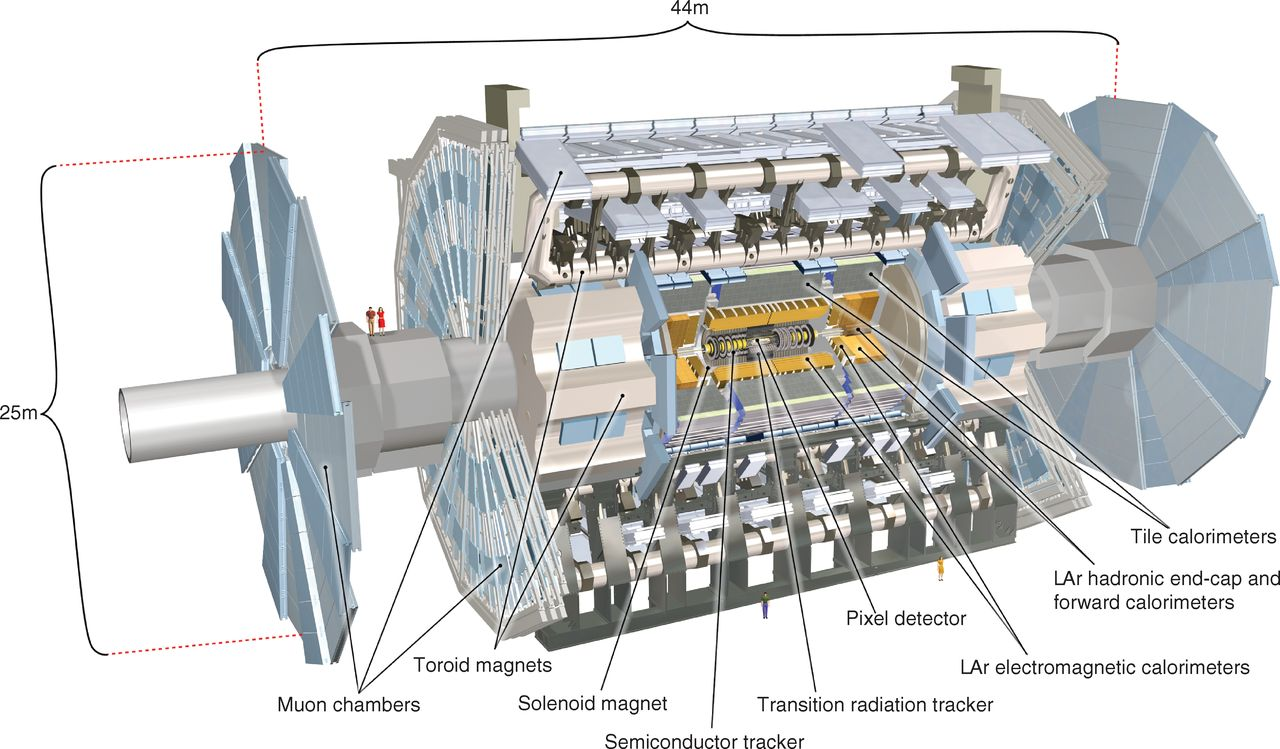
\includegraphics[width=16.0cm]{physics/atlas_detector.jpg}
	
	\caption{Slika s prečnim prerezom detektorja ATLAS, ki prikazuje njegove glavne komponente \cite{AadScience2012}.  }
	\label{detektoratlas}
\end{figure}

Zgradba detektorja, ki v višino meri 25, v dolžino pa 44 metrov, je prikazana na sliki \ref{detektoratlas}. Zgrajen je iz velikega števila komponent, ki so potrebne za merjenje produktov, ki nastanejo ob trkih. Notranji detektor (\textit{inner detector}, ID) zaznava sledi nabitih delcev, ki so ukrivljene zaradi magnetnega polja tankih selenoidnih magnetov. V srednji plasti se nahajata dva kalorimetra, elektromagnetni (EM) in hadronski, ki merita energijo delcev. Na zunanji strani mionski spektrometer (MS) beleži sledi mionov, ki se ukrivijo zaradi magnetnega polja superprevodnih toroidnih magnetov.

Elektron v sredici pusti sled in se zaustavi v elektromagnetnem kalorimetru. Foton se obnaša podobno, le da v sredici ne pusti sledi. Proton pusti sled, interagira pa v hadronskem kalorimetru. Nevtron se obnaša podobno, a za seboj ne pušča sledi. Mion potuje skozi detektor in za seboj pušča sled (v ID in MS). Nevtrino pa potuje skozi detektor ATLAS ne da bi ga le-ta zaznal \cite{CerknLHCParticles}.

Vsak dogodek vsebuje v končnem stanju približno 10 delcev, ki nas zanimajo. Lastnosti delcev se rekonstruirajo iz stotin surovih signalov detektorja. V diplomskem delu med relevantne delce spadajo: elektroni, mioni, hadronski tau, pljuski (\textit{jets}) in manjkajoča prečna energija. Elektron, mion in delec $\tau$ so trije leptoni iz standardnega modela. Življenjska doba elektronov in mionov je dovolj velika, da lahko ti delci dosežejo detektorje. Zaradi tega je mogoče njihove lastnosti (energijo in smer) izmeriti neposredno. Delci $\tau$ razpadejo skoraj hipoma, bodisi v elektron in dva nevtrina, bodisi v mion in dva nevtrina ali skoraj kolinearni pljusk nabitih delcev in nevtrino. Pljusk imenujemo tudi hadronski tau.  Izmerjena gibalna količina vseh delcev v dogodku je najpomembnejša informacija, ki je na voljo pri klasifikaciji dogodkov.

Namesto koordinate $\theta$ pogosto uporabimo \textit{psevdorapidnost} (glej enačbo \ref{eq:pseudorapidity}). Vrednost $\eta = 0$ opisuje delec v $x\text{-}y$ ravnini ($\theta = \pi/2$), $\eta = +\infty$ pa ustreza delcu, ki potuje vzdolž osi $z$ ($\theta = 0$). Delec, ki potuje v nasprotni smeri ima $\eta = -\infty$. Delce je možno v celoti identificirati (in jim določiti gibalno količino) v razponu psevdorapidnosti $\eta \in \left[-\num{2,5}; \num{2,5} \right]$. Pri vrednostih $|\eta| \in \left(\num{2,5}; 5\right]$ delcev v detektorju ni več mogoče identificirati, je pa moč izmeriti njihovo gibalno količino. Delcev z $|\eta| > 5$ ni možno zaznati.

Rekonstrukcijo in identifikacijo leptonov, pljuskov in manjkajoče prečne energije v detektorju ATLAS izvedejo s pomočjo standardnih algoritmov. Potrebne podatke za \textbf{rekonstrukcijo elektrona} pridobijo iz EM kalorimetra in sledi v notranjem detektorju. Pri \textbf{rekonstrukciji mionov} si ne morejo pomagati s podatki iz kalorimetra, pač pa podatkom iz ID detektorja dodajo še podatke o sledi iz mionskega spektrometra v zunanjem delu detektorja. Odvisno od $\eta$ in $p_T$ je uspešnost algoritmov za detekcijo obeh leptonov med $80\mbox{-}90\%$, uporabljati pa morajo še različne filtre za nezaželene podobne dogodke. \textbf{Pljuske rekonstruirajo} iz podatkov hadronskega kalorimetra, pri čemer upoštevajo tudi pripadajoče topološke podatke. Pljuski so namreč skoraj kolinearni. Uspešnost algoritma je $60\mbox{-}70\%$, pri tem pa se lahko v do $\num{0,5}\%$ primerih zgodijo tudi napake pri klasifikaciji. \cite{atlas2013}.

Nevtrinov, ki nastanejo ob razpadu delca $\tau$, detektor ne zazna. O njihovih lastnostih lahko sklepamo na podlagi zakona o ohranitvi gibalne količine. Veliko delcev, ki se pomikajo vzdolž osi $z$ ($|\eta| > 5$), tudi uide detekciji. Zaradi tega vsoto gibalnih količin delcev, ki jih nismo uspeli zaznati, izračunamo le v prečni ravnini, predstavlja pa jo dvodimenzionalni vektor $\mathbf{E^{miss}_T}$.

Invariantno maso kandidata za Higgsov bozon rekonstruirajo s pomočjo posebne metode (\textit{missing mass calculator}, MMC), ki je podrobneje razložena v \cite{tautaumassrecon}. Metoda rešuje poddeterminiran sistem enačb 6 do 8 neznank (odvisno od števila nevtrinov v končnem stanju). Neznanke vsebujejo komponente gibalne količine, ki jo nosijo nezaznani nevtrini vsakega od leptonov $\tau$, in invariantni masi nevtrinov leptonskega razpada $\tau$. Metoda upošteva omejitve, ki jih prinašajo izmerjene količine v smereh $x$ in $y$. V naslednjem koraku metoda naredi vzorčenje preko prostih neznank in za vsako točko izračuna utež, ki temelji na verjetnosti obstoja takega stanja glede na topologijo razpada $\tau$. Sistem vrne najbolj verjetno oceno mase kandidata za Higgsov bozon.


% -----------------------------------------------------------------------------
% POGLAVJE: Opredelitev problema
% -----------------------------------------------------------------------------
\chapter{Opredelitev problema}

Problem, s katerim sem se spopadel v diplomskem delu, sledi formulaciji na odprtem tekmovanju \textit{The Higgs Boson Machine Learning Challenge (HiggsML)}\footnote{ \url{http://www.kaggle.com/c/higgs-boson}}, ki temelji na rezultatih kolaboracije ATLAS \cite{Adam-Bourdarios14}. Poenostavitev naloge glede na polni problem pri ločevanju signala in ozadja v eksperimentu ATLAS je razložena v uvodnih poglavjih diplomskega dela.

\section{Formalna opredelitev problema}

Naj ${\cal D} = \left\{({\mathbf x}^{(1)}, y^{(1)}, w^{(1)}), \dots, ({\mathbf x}^{(n)}, y^{(n)}, w^{(n)}) \right\}$ predstavlja učno podatkovno množico, kjer je $\mathbf{x}^{(i)} \in \mathbb{R}^d$ $d$-dimenzionalni vektor značilk, $y^{(i)} \in \{\text{b, s}\}$ je oznaka, $w^{(i)} \in \mathbb{R}^+$ pa je nenegativna utež. Oznaka $\text{b}$ označuje ozadje (ang. \textit{background}), $\text{s}$ pa signal. Naj bosta ${\cal S} = \{i : y^{(i)} = \text{s}\}$ in ${\cal B} = \{i : y^{(i)} = \text{b}\}$ množici indeksov dogodkov, ki predstavljajo signal in ozadje, $n_\text{s} = |{\cal S}|$ in $n_\text{b} = |{\cal B}|$ pa naj označujeta število dogodkov. Z dvignjenimi indeksi v oklepaju so označene količine v podatkovni množici, npr. z $\mathbf{x}^{(i)}$ je zapisan $i$-ti vektor značilk, s spuščenimi indeksi pa so označene komponente vektorjev, npr. $j$-ta komponenta vektorja značilk je zapisana z $x_j$.

Podatki, na katerih se učimo, so simulirani (glej poglavje \ref{analiza-podatkov}) in se razlikujejo od izmerjenih. Razmerje $n_\text{s} / n_\text{b}$ v podatkih tako ne odraža dejanskega razmerja dogodkov $P(y = s) / P(y = b)$. Glede na nizko verjetnost, da pri nekem naravnem dogodku gre za signal \cite{Adam-Bourdarios14}, je tako učna podatkovna množica precej bolj uravnotežena in omogoča metodam, da se lahko naučijo razlikovati med dogodki, ki predstavljajo ozadje in tistimi, ki predstavljajo signal.

Podatek, ki ga da simulacija, je tudi utež $w^{(i)}$, ki je mera za verjetnost nekega dogodka v dejanskem eksperimentu. Ker je optimizacijska funkcija (\ref{en:ams}) odvisna od \textit{nenormalizirane vsote} uteži in ker želimo, da je naš sistem invarianten na števili simuliranih dogodkov $n_s$ in $n_b$, moramo vsoto vsake podatkovne množice (učne, potrjevalne ali testne) za vsak razred (signal ali ozadje) fiksirati:
\begin{equation}
\sum_{i \in \cal{S}}{w^{(i)}} = N_s
\qquad\text{in}\qquad
\sum_{i \in \cal{B}}{w^{(i)}} = N_b
\label{eq:sumweights}
\end{equation}
Normalizacijski konstanti $N_s$ in $N_b$ imata fizikalni pomen in predstavljata \textit{pričakovano število} dogodkov, ki predstavljajo signal in ozadje v obdobju zajema podatkov na LHC (v našem primeru leta 2012). Individualne uteži so proporcionalne pogojnim gostotam, deljenimi z instrumentalnimi gostotami, uporabljenimi na simulatorju.
\begin{equation}
	w^{(i)} = \left\{\begin{array}{r}
		p_s(\textbf{x}^{(i)})/q_s(\mathbf{x}^{(i)}),\qquad \text{če}\;y^{(i)} = \text{s} \\
		p_b(\textbf{x}^{(i)})/q_b(\mathbf{x}^{(i)}),\qquad \text{če}\;y^{(i)} = \text{b} 
	\end{array}
	\right.,
	\label{eq:weightseparation}
\end{equation}
kjer sta
\begin{equation*}
p_s(\textbf{x}^{(i)}) = p(\textbf{x}^{(i)}|y = \text{s}) \qquad \text{in} \qquad p_b(\textbf{x}^{(i)}) = p(\textbf{x}^{(i)}|y = \text{b})
\end{equation*}
pogojni gostoti signala in ozadja ter $q_s(\textbf{x}^{(i)})$ in $q_b(\textbf{x}^{(i)})$ instrumentalni gostoti.

Naj bo $g : \mathbb{R}^d \rightarrow \{\text{b, s}\}$ poljubna klasifikacijska funkcija. Naj bo izbrano področje ${\cal G} = \{\textbf{x} : g(\textbf{x}) = \text{s}\}$ množica točk, klasificirana kot signal, in naj $\hat{\cal G}$ označuje množico indeksov točk, ki jih $g$ izbere (klasificira kot signal).
\begin{equation*}
\hat{\cal G} = \{ i : \textbf{x}^{(i)} \in {\cal G}\} = \{ i : g(\textbf{x}^{(i)}) = \text{s} \}.
\end{equation*}
Iz enačb \ref{eq:sumweights} in \ref{eq:weightseparation} sledi, da je količina
\begin{eqnarray}
	s = \sum_{i \in {\cal S} \cap {\hat{\cal G}}} w^{(i)}
	\label{eq:s}
\end{eqnarray}
nepristranska ocena pričakovanega števila dogodkov signala, ki ga izbere klasifikacijska funkcija $g$,
\begin{eqnarray}
	\mu_s = N_s \int_{\cal G}p_s(\mathbf{x})d\mathbf{x}.
\end{eqnarray}
Na podoben način je
\begin{eqnarray}
	b = \sum_{i \in {\cal B} \cap {\cal G}} w^{(i)}
	\label{eq:b}
\end{eqnarray}
nepristranska ocena pričakovanega števila dogodkov ozadja, izbranih s pomočjo klasifikatorja $g$,
\begin{eqnarray}
	\mu_b = N_b \int_{\cal G}p_b(\mathbf{x})d\mathbf{x}.
\end{eqnarray}
V terminologiji strojnega učenja sta količini $s$ in $b$ nenormalizirani oceni pravilno pozitivnih in pravilno negativnih primerov (glej razdelek \ref{sec:ml_eval}).

\section{AMS metrika}
\label{sc:ams}
Glede na klasifikator $g$ je metrika za oceno uspešnosti definirana kot ciljna funkcija $AMS$ (\textit{approximate median significance})
\begin{equation}
\text{AMS} = \sqrt{2 \left( ( s + b + b_{reg} ) \ln \left( 1 +  \frac{s}{b + b_{reg}} \right) - s \right) },
\label{en:ams}
\end{equation}
kjer sta $s$ in $b$ definirana z enačbama \ref{eq:s} in \ref{eq:b}, $b_{reg}$ pa je regularizacijska količina, nastavljena na konstantno vrednost $b_{reg} = 10$.

Rešitev problema predstavlja implementacija klasifikatorja $g$, ki ga naučimo s pomočjo učne podatkovne množice ${\cal D}$, in sicer tako, da maksimiziramo $AMS$ na potrjevalni podatkovni množici.

% -----------------------------------------------------------------------------
% POGLAVJE: Metode strojnega učenja
% -----------------------------------------------------------------------------
\chapter{Uporabljene metode strojnega učenja}

Strojno učenje predstavlja področje računalništva, ki se ukvarja z vprašanjem oblikovanja računalniških programov, katerih funkcija se samodejno izboljšuje z novimi izkušnjami \cite{Mitchell1997, Witten2005}. Med glavne rešitve, ki jih v vsakodnevnem življenju dandanes prinaša strojno učenje, spadajo denimo filtri nezaželene elektronske pošte, programi za odkrivanje zlorab pri finančnih transakcijah, priporočilni sistemi, ki nam predlagajo za nas zanimive novice za branje ali izdelke za nakup ... V tehniki se velikokrat srečujemo z algoritmi za napovedovanje določenih časovnih vrst (npr. cene ali rabe energije) in klasifikacijo dogodkov (npr. ali je nek izdelek v proizvodnem procesu brez napak).

V tem poglavju so predstavljene metode, ki so relevantne predvsem za reševanje problema klasifikacije meritev detektorja ATLAS: raziskovalna analiza podatkov in klasifikacijske metode, ki so del širše družine metod nadzorovanega učenja. 

\section{Raziskovalna analiza podatkov}
Raziskovalna analiza podatkov predstavlja enega od pristopov k začetni analizi množice podatkov predvsem s pomočjo vizualnih metod. Vizualne metode temeljijo na sposobnosti človeških možganov, da prepoznajo strukturo v podatkih. Namen analize je pregledati osnovne lastnosti podatkov, ki pomagajo pri določanju scenarijev za implementacijo metod strojnega učenja. Poleg tega so vizualne metode na področju rudarjenja podatkov pomembne tudi zato, ker je mogoče z njihovo pomočjo odkriti nove, nepričakovane zakonitosti v podatkih. Metode raziskovalne analize imajo pri visoko-dimenzionalnih naborih podatkov očitne omejitve. Opisi v diplomskem delu so, kjer ni drugače navedeno, povzeti po \cite{hand2001}.

Opisani pristop temelji na podatkih in ne na predhodnem domenskem znanju. Metodologija je bila razvita že v začetku šestdesetih let prejšnjega stoletja, je pa svoj preporod doživela z razvojem računalništva, ki je močno olajšalo izdelavo vizualizacij. 

\textbf{Osnovni pregled značilk} se nanaša na pregled po eni značilki. Zajema \textbf{pregled manjkajočih vrednosti} v podatkih, \textbf{pregled osnovnih agregatov} in natančnejši \textbf{pregled porazdelitev} določenih značilk s pomočjo histogramov. Pregled osnovnih agregatov zajema: povprečja, standardno deviacijo, minimum, maksimum, število vrednosti, kvantile ... Ponazoritev posameznih značilk s pomočjo histogramov pa nam da lepši grafični pregled in informacijo o porazdelitvi posamezne značilke.

\textbf{Razpršeni grafi} se nanašajo na 2 značilki. Podatke ponazorimo s točkami, katerih koordinate predstavljajo vrednosti obeh značilk. Grafe ponavadi prikažemo v matriki 2, 3 ali 4 različnih značilk, tako da jih lahko primerjamo med sabo. Takšen prikaz nam lahko razkrije skrito strukturo v podatkih, ki je po pregledu ene same značilke ne zasledimo. V primeru klasifikacije lahko npr. opazimo, če določena kombinacija značilk bolje loči oba razreda kot ena sama. Opazimo lahko tudi medsebojno korelacijo posameznih značilk, ki se odraža na urejenosti/razpršenosti točk.

\textbf{Korelacijska matrika značilk} je zelo učinkovita metoda za hiter in celosten pregled nad podatki. V matriki dimenzije $d \times d$, kjer je $d$ število značilk, s pomočjo barvne lestvice ponazorimo korelacijo med parom značilk. S pomočjo kompletnega pivotiranja, ki ga naredimo s hierarhičnim grozdenjem, lahko značilke, ki so si med seboj podobne, smiselno uredimo. Metoda je še zlasti uporabna pri izločanju linearno odvisnih značilk, ki modelom ne prinašajo dodatne vrednosti. 

\textbf{Analiza glavnih komponent} je definirana kot ortogonalna linearna transformacija, ki transformira nabor podatkov v nov koordinatni sistem, in sicer tako, da komponenta z največjo varianco neke projekcije podatkov leži na prvi koordinati, druga največja na drugem mestu in tako naprej. Metoda je poenostavitev metode večrazsežnega skaliranja.

Praktična uporaba opisanih metod z rezultati na podatkih iz detektorja ATLAS je opisana v poglavju \ref{analiza-podatkov}.

\section{Metode za nadzorovano učenje}

Na področju strojnega učenja v grobem ločimo dva različna razreda metod: (1) \textbf{metode za nadzorovano učenje} in (2) \textbf{metode za nenadzorovano učenje}. Slednji se ponavadi izvaja na podatkih, ki ne vsebujejo oznake $y^{(i)}$, torej parametra, ki nas zanima. Zakonitosti iščemo torej samo v strukturi, ki jo oblikuje množica točk $x^{(i)}$ v faznem prostoru. Osnovni primer take metode je grozdenje, ki poskuša točke glede na izbrano definicijo razdalje povezati v smiselne zaključene množice - grozde. Metoda grozdenja je lahko tudi učinkovita metoda generiranja novih značilk, pri čemer oznaka grozda služi kot dodatna značilka v nadzorovanem učnem problemu.

Metode za nadzorovano učenje delujejo na podatkih z znanim parametrom, ki nas zanima ($y^{(i)}$). Ločimo regresijske in klasifikacijske metode. Pri \textbf{regresijskih metodah} je ponavadi parameter $y^{(i)} \in \mathbb{R}$. Cilj regresijskih metod je za neznano točko $x^{(i)}$ oceniti realno vrednost $y^{(i)}$. 

V tipičnem \textbf{klasifikacijskem problemu}, ki je tudi sicer predmet diplomskega dela, imamo množico vektorjev v prostoru $x^{(i)} \in \mathbb{R}^d$ (vektor značilk) in pripadajočih oznak $y^{(i)} \in \{1, 2, 3, \ldots, N\}$, kjer $N$ označuje število različnih razredov. Oznaka $y^{(i)}$ nam pove, v kateri razred spada vektor $x^{(i)}$. Cilj klasifikacijskega problema je predvideti oznake neznanih vektorjev, in sicer tako, da bo pri tem napaka najmanjša.

Za binarne klasifikacijske probleme velja $N = 2$. V takih primerih obstajata 2 razreda: pozitivni in negativni. S takšnim problemom se srečujemo tudi v tem diplomskem delu.


\section{Pregled klasifikacijskih metod}

Pri pregledu klasifikacijskih metod sem se omejil na naslednje metode: osnovne metode, ki prinašajo dodaten vpogled v podatke (logistična regresija), osnovne metode, ki jih je predlagal organizator (preprosto okno), zmagovalno metodo (pospešena odločitvena drevesa) in na metodo, katere uporabo za dani problem sem želel v diplomskem delu sam raziskati - metodo podpornih vektorjev. Teoretični pregled metod temelji predvsem na \cite{AndrewNgML}.


\subsection{Logistična regresija}

Linearno regresijo je moč, ko imamo opravka z numeričnimi značilkami, uporabiti kot klasifikacijsko metodo. Pravzaprav lahko vsako regresijsko tehniko uporabimo za klasifikacijo. Prenos regresijske tehnike v klasifikacijsko domeno lahko naredimo s pomočjo preprostega trika, in sicer da pozitivno klasificiranim točkam pripišemo vrednost 1, negativno klasificiranim pa vrednost 0. Ko poskusimo s pomočjo naučenega modela klasificirati neznano točko, lahko vrednost, ki jo vrne linearna regresija, interpretiramo kot funkcijo članstva v določenem razredu \cite{Witten2005}.

Težava tega pristopa je, da se funkcija članstva ne nanaša na verjetnost pripadnosti vzorca določenemu razredu (saj je lahko večja od 1 ali manjša od 0), hkrati pa je binarna porazdelitev vrednosti točk daleč od normalne, ki jo zahteva metoda.

\textit{Logistična regresija} je statistična metoda, ki nima težav iz zgornjega odstavka. Namesto, da bi poskusila vrednosti 0 in 1 aproksimirati neposredno, uporabi za ta namen transformacijsko funkcijo ($[0, 1] \rightarrow \mathbb{R}$). Katerokoli realno število pretvori na interval med 0 in 1.

Standardno logistično funkcijo zapišemo kot
\begin{equation}
	\label{en:standardna_log_funkcija}
	h_\theta(x) = g(\theta^Tx) = \frac{1}{1 + e^{-\theta^Tx}},
\end{equation}
kjer se
\begin{equation}
	g(z) = \frac{1}{1 + e^{-z}}
\end{equation}
imenuje \textbf{logistična funkcija} ali \textbf{sigmoid}. $h(x)$ predstavlja linearno kombinacijo značilk $h(x) = \theta_0 + \theta_1x^{(1)} + \theta_2x^{(2)} + \dots + \theta_nx^{(n)}$. Če privzamemo $x_0^{(i)} = 1$, lahko zapišemo $h(x) = \theta \cdot x$.

Interpretacija hipoteze je verjetnostna. Vrednost hipoteze je $P(y=1|x;\theta)$ - torej verjetnost, da je $y = 1$ pri danem $x$ in $\theta$.

Naloga učnega algoritma je določitev parametrov $\theta_i$. Najprej moramo definirati logistično minimizacijsko funkcijo $J(\theta)$. Ta funkcija je odvisna od razlike med hipotezo in dejansko vrednostjo točk. Pri linearni regresiji funkcijo zapišemo kot
\begin{equation}
	J(\theta) = \frac{1}{m} \sum^m_{i = 1} \frac{1}{2} \left( h_\theta(x^{(i)}) - y^{(i)}\right)^2.
\end{equation}
Parameter $\theta$ določimo tako, da je vsota kvadratnih členov najmanjša. Pri logistični regresiji sumand nadomestimo s stroškovno funkcijo $\text{Cost}(h_\theta(x), y)$. Zapišimo stroškovno funkcijo
\begin{equation}
	\text{Cost}(h_\theta(x), y) = \left\{
	\begin{array}{rl}
		-\log(h_\theta(x)) & \text{če je} \; y = 1 \\
		-\log(1 - h_\theta(x)) & \text{če je} \; y = 0
	\end{array}
	\right.
\end{equation}
Vemo, da je $y \in \{0, 1\}$. Zdaj lahko v eni sapi zapišemo $J(\theta)$
\begin{equation}
	J(\theta) = -\frac{1}{m} \left[ 
		\sum^m_{i = 1}
			y^{(i)} \log h_\theta(x^{(i)}) + (1 - y^{(i)}) \log (1 - h_\theta(x^{(i)}))
	\right].
	\label{en:j_theta}
\end{equation}
Naša učna naloga je poiskati tak $\theta$, da bo $J(\theta)$ najmanjši. Napoved za nov nepoznani $x$ izračunamo s pomočjo enačbe (\ref{en:standardna_log_funkcija}), ki nam predstavlja verjetnost, da dani primerek spada v pozitivni razred $P(y = 1 | x;\theta)$. $\theta$ bomo poiskali s pomočjo minimizacije $J(\theta)$, in sicer s pomočjo gradientnega spusta.

Ena pomembnih tehnik pri zagotavljanju uspešnega gradientnega spusta je skaliranje značilk. S tem se izognemo nepotrebnim oscilacijam, ki upočasnjujejo konvergenco. Oscilacije so posledica dejstva, da je velikostni red nekaterih značilk precej nižji ali višji od ostalih.

Osnovni algoritem gradientnega spusta je zelo preprost. Potrebno je izračunati parcialne odvode $\frac{\partial}{\partial x_i}J(\theta)$. Upoštevajoč enačbo (\ref{en:j_theta}) lahko zapišemo posamezni korak naše minimizacije
\begin{equation}
	\theta_j := \theta_j - \alpha \sum^m_{i = 1}(h_\theta(x^{(i)}) - y^{(i)})x_j^{(i)},
	\label{en:log_reg_update}
\end{equation}  
pri čemer velja $j \in \{1, 2, \ldots, d\}$, popravki pa se izvršijo simultano (torej ne vplivajo drug na drugega).



\subsection{Metoda podpornih vektorjev}

Denimo, da imamo binarni klasifikacijski problem in da sta razreda točk v našem prostoru linearno separabilna. V večini takih primerov obstaja neskončno mnogo različnih hiperravnin, ki ločujejo med sabo oba razreda (glej sliko \ref{svmseparable}).

\begin{figure}[ht]
	\includegraphics[width=5.2cm]{methods/svm/svm_axes_1.pdf}
	\includegraphics[width=5.2cm]{methods/svm/svm_axes_2.pdf}
	\includegraphics[width=5.2cm]{methods/svm/svm_axes_3.pdf}	
	
	\caption{Veliko različnih rešitev za hiperravnino, ki ločuje razreda primerkov.}
	\label{svmseparable}
\end{figure}

Metoda podpornih vektorjev (\textit{angl. Support Vector Machine} oz. SVM) se imenuje tudi klasifikator maksimalnega razmika. Prej opisani problem binarne klasifikacije s tem dobi enolično rešitev. Primer klasifikatorja z maksimalnim razmikom je ilustriran na sliki \ref{sl:svmmaxclass}.

\begin{figure}[h!]
	\centering
	\setlength{\unitlength}{1cm}
	\begin{picture}(10,8)
	% separating plane
	\color{black}
	\put(1, 1){	\line(1, 1){6} }
	\color{blue}
	\put(0, 1.5){ \line(1, 1){6} }
	\put(2, 0.5){ \line(1, 1){6} }
	
	\color{black}
	\put(6.63, 6.5){\vector(1, -1){0.76}}
	\put(7.29, 5.84){\vector(-1, 1){0.67}}
	\put(7.45, 6.55){\makebox(0,0){razmik}}
	\put(2, 2.4){\rotatebox{45}{ločujoča}}	
	\put(2.2, 1.6){\rotatebox{45}{hiperravnina}}		
	
	% green class	
	\color{green}
	\put(1, 7){\circle{0.1}}
	\put(2.5, 6){\circle{0.1}}
	\put(3, 5){\circle{0.1}}
	\put(1.2, 3.3){\circle{0.1}}
	\put(5.2, 7.5){\circle{0.1}}
	\put(0.7, 5.3){\circle{0.1}}
	\put(2.5, 4.8){\circle{0.1}}
	\put(4.2, 7){\circle{0.1}}


	\put(5.63, 7){\circle{0.1}}
	\put(2.63, 4){\circle{0.1}}
	\put(1.63, 3){\circle{0.1}}
	
	% red class
	\color{red}
	\put(5.63, 4){\circle{0.1}}
	\put(2.63, 1){\circle{0.1}}
	
	\put(5, 0.7){\circle{0.1}}
	\put(7, 4.7){\circle{0.1}}
	\put(5, 2.7){\circle{0.1}}
	\put(3.5, 1.4){\circle{0.1}}
	\put(2.5, 0.4){\circle{0.1}}
	\put(6, 3.2){\circle{0.1}}
	\put(5.5, 1.9){\circle{0.1}}
	\put(4.5, 1.4){\circle{0.1}}
	\put(6.5, 2.9){\circle{0.1}}
	
	\end{picture}
	\caption{Maksimalni razmik ločujoče hiperravnine pri metodi podpornih vektorjev.}
	\label{sl:svmmaxclass}
\end{figure}

Hiperravnino, ki ločuje različna razreda primerkov označimo s $H$. Enačbo ravnine lahko zapišemo kot
\begin{equation}
  H(w, b) = w^T x + b = 0,
\end{equation}
kjer je $w$ normalni vektor (v našem kontekstu ga bomo imenovali \textit{vektor uteži}), $b$ pa odmik ravnine v izhodišču. Opazimo, da v primeru množenja obeh parametrov z enakim pozitivnim koeficientom dobimo enako hiperravnino. Za enolično reprezentacijo hiperravnine je potrebno zato normalizirati faktorja $w$ in $b$ glede na podatke iz učne podatkovne množice. Reprezentaciji z normaliziranima $w$ in $b$ pravimo tudi kanonična reprezentancija.

Formalno zapišemo
\begin{equation}
	\min |w^T x + b| = 1
\end{equation}
in glede na prejšnji odstavek definiramo dva podporna vektorja v točkah $(x^{(1)}, 1)$ in $(x^{(2)}, -1)$:
\begin{eqnarray}
	w^Tx^{(1)} + b &=& 1 
	\label{eq:svm_vectors_1} \\
	w^Tx^{(2)} + b &=& -1
	\label{eq:svm_vectors_minus1}
\end{eqnarray}
Razdaljo med neko točko $x$ in hiperravnino $H$ izračunamo s pomočjo
\begin{eqnarray}
	d(x, H(w, b)) = \frac{w^Tx + b}{||w||}.
	\label{eq:svm_distance}
\end{eqnarray}
Cilj metode je maksimizirati razdaljo med podpornima vektorjema glede na $w$ in $b$. Upoštevajoč enačbe \ref{eq:svm_vectors_1}, \ref{eq:svm_vectors_minus1} in \ref{eq:svm_distance}, lahko izračunamo razmik, ki je $2 / ||w||$. Pri metodi podpornih vektorjev želimo ta razmik maksimizirati, kar pomeni, da moramo minimizirati $||w||$, kar je ekvivalentno minimizaciji $||w^2||/2$. Pri tem velja robni pogoj $y^{(i)}(w^Tx^{(i)} + b) > 1$ za $i = 1, 2, \ldots, n$. Takšen problem znamo rešiti z uporabo Lagrangeovih multiplikatorjev $\alpha_i$. Zapišimo Lagrangeovo funkcijo
\begin{eqnarray}
	L(w, b, \alpha) = \frac{1}{2}||w||^2 - \sum^n_{i=1} \alpha_i(y^{(i)}(w^Tx^{(i)} + b) - 1),
\end{eqnarray}
kjer je $y^{(i)} \in \{-1, 1\}$ oznaka razreda točke $x^{(i)}$. Prvi del funkcije poskrbi za maskimizacijo razmika, drugi del pa za minimizacijo napake pri učenju.

Zanimajo nas parcialni odvodi Lagrangeve funkcije, ki jih postavimo na nič: $\frac{d}{db}L(w, b, \alpha) = 0$ in $\frac{d}{dw}L(w, b, \alpha)$. Dobimo
\begin{eqnarray}
	\sum^n_{i=1}\alpha_iy^{(i)} = 0 \qquad \text{in} \qquad
	w = \sum^n_{i=1}\alpha_iy^{(i)}x^{(i)}.
	\label{eq:svm_w}
\end{eqnarray}
Lagrangeovo funkcijo in zadnji rezultat lahko uporabimo za formulacijo t. i. Lagrangeovega dualnega problema, s katerim izračunamo $\alpha_i$. Zapišemo dualno Lagrangeovo funkcijo
\begin{eqnarray}
	D(\alpha) = \sum^n_{i=1} \alpha_i - \frac{1}{2}\sum^n_{i=1} \sum^n_{j=1} \alpha_i\alpha_j y^{(i)}y^{(j)} \left<x^{(i)},x^{(j)} \right>,
	\label{eq:svm_dual_lagrange}
\end{eqnarray}
pri čemer velja $\alpha_i \geq 0$ in $\sum^n_{i=1}\alpha_iy^{(i)} = 0$.

Z minimizacijo \ref{eq:svm_dual_lagrange} dobimo vrednosti koeficientov $\alpha_i$, ki jih uporabimo za izračun vektorja $w$, pri čemer uporabimo enačbo \ref{eq:svm_w}. Klasifikacijsko funkcijo lahko enostavno zapišemo kot
\begin{eqnarray}
	g(x) = \text{sign} \left(\sum^n_{i=1} \alpha y^{(i)} \left<x^{(i)},x\right> + b\right).
\end{eqnarray}

\subsubsection{Mehki razmik}
Kljub transformaciji značilk v visoko-dimenzionalni prostor je včasih nemogoče najti hiperravnino, ki bi lahko ločila med seboj primere različnih razredov iz učne množice podatkov. V takem primeru, je mogoče uporabiti metodo mehkega razmika, ki bo ob upoštevanju morebitne napake v klasifikaciji znala poiskati tako hiperravnino. 

Problem lahko preprišemo v minimizacijo izraza $||w||^2 + C\sum^n_{i=1}\xi_i$, pri čemer velja robni pogoj $y^{(i)}(w^Tx^{(i)} + b) > 1 - \xi_i$, za $i = 1, 2, ..., n$, kjer je $\xi$ označuje mero za napačno klasifikacijo, $C$ pa je parameter, ki nadzira vpliv $\xi$. Izbira regularizacijskega parametra $C$ ima velik vpliv na končni rezultat.

\subsubsection{Jedra in projekcija v prostor z več dimenzijami}
Separabilnosti primerov v učni množici včasih ni mogoče doseči v prostoru značilk. Metoda omogoča projekcijo iz nizko-dimenzionalnega prostora značilk v visoko-dimenzionalni prostor s pomočjo uporabe t. i. jeder. Uporaba jeder temelji na uporabi skalarnega produkta $\left<x^{(i)}, x^{(j)}\right>$ v formulaciji dualnega problema iz enačbe \ref{eq:svm_dual_lagrange}. 

Denimo, da imamo funkcijo $\phi$, ki preslika značilko $x$ v visoko-dimenzionalni prostor $\mathbb{R}^{N_v}$, pri čemer je $N_v$ število dimenzij tega prostora. Z uporabo jeder $K$, ki so definirana v nizko-dimenzionalnem prostoru značilk, se izognemo včasih težavnemu izračunu skalarnega produkta v visoko-dimenzionalnem prostoru.

Jedro $K$ je definirano z
\begin{eqnarray}
	K(x^{(p)}, x^{(q)}) = \left<\phi(x^{(p)}), \phi(x^{(q)})\right>,
\end{eqnarray}
kjer sta $x^{(p)}$ in $x^{(q)}$ definirana v prostoru značilk. Za jedro $K$ velja nekaj posebnih lastnosti (Mercerjev teorem): mora biti pozitivno definitno in simetrično. Zdaj lahko formulacijo dualnega problema iz \ref{eq:svm_dual_lagrange} prepišemo v 
\begin{eqnarray}
	W(\alpha) = \sum^n_{i = 1}\alpha_i - \frac{1}{2} \sum^n_{i=1} \sum^n_{j=1} \alpha_i \alpha_j K(x^{(i)}, x^{(j)}),
\end{eqnarray}
klasifikacijsko funkcijo pa v
\begin{eqnarray}
	g(x) = \text{sign} \left(\sum^n_{i=1}\alpha y_i K(x^{(i)}, x) + b \right).
\end{eqnarray}

Obstaja veliko tipov jeder, med najbolj običajne spadajo:
\begin{itemize}
	\item linearno: $K(x^{(i)}, x^{(j)}) = x^{(i)T}x^{(j)}$
	\item polinomsko: $K(x^{(i)}, x^{(j)}) = (\gamma x^{(i)T}x^{(j)} + c)^d$, $\gamma > 0$ 
	\item gaussovsko (RBF - \textit{radial basis function}): $K(x^{(i)}, x^{(j)}) = \exp(-\gamma |x^{(i)}-x^{(j)}|^2)$, $\gamma > 0$ 
\end{itemize}

\subsection{Odločitvena drevesa}
\label{sc:decisiontrees}
Odločitvena drevesa (s tem mislimo na njihovo učenje) so metoda za aproksimacijo diskretnih funkcij. Naučena funkcija je predstavljena s pomočjo odločitvenega drevesa \cite{Mitchell1997}. 

Odločitvena drevesa klasificirajo različne primere tako, da jih razporedijo v drevesno obliko od korena do listov. Vsako vozlišče v drevesu definira test določene značilke, vsaka veja, ki iz tega vozlišča izhaja, ustreza določenim vrednostim te značilke. Klasifikacijo določenega primera pričnemo pri korenu. Glede na izid vozliščnega testa se pomaknemo v eno od vej. Postopek ponavljamo, dokler ne dosežemo končnega vozlišča (lista).

Na sliki \ref{sl:algo-id3} je prikazan algoritem \texttt{ID3}, prilagojen učenju diskretnih funkcij. Algoritem gradi drevo od korena proti listom. V vsakem vozlišču izbere značilko, ki najbolje klasificira lokalno učno množico. Proces se izvaja, dokler se naučeno drevo v popolnosti ne prilagaja učni množici ali do izrabe vseh značilk.

\SetStartEndCondition{ }{}{}
\SetKwProg{Fn}{function}{\string:}{}
\SetKwFunction{FRecurs}{ID3}

\begin{figure}[h!]
	\begin{algorithm}[H]				
		\Fn{\FRecurs{${\cal D}$, ${\cal A}$}}{								
			${\cal D}$ je učna množica podatkov\;
			${\cal A}$ je množica značilk za klasifikacijo\;
			če ${\cal D}$ vsebuje le pozitivne primere, vrni drevo s korenskim vozliščem z oznako +\;
			če ${\cal D}$ vsebuje le negativne primere, vrni drevo s korenskim vozliščem z oznako -\;
			če ${\cal A}$ ne vsebuje nobenih značilk, vrni drevo s korenskim vozliščem z najbolj pogosto oznako primerov\;
			\Begin{
				izberi značilko $Z$, ki najbolje klasificira primere iz {\cal D}\;
				odločitveni atribut za korensko vozlišče je $Z$\;
				\For{vse možne vrednosti $v_i$ značilke $Z$\,} {
					dodaj novo vejo, ki ustreza testu $Z = v_i$\;
					naj bo ${\cal D}_{v_i}$ podmnožica ${\cal D}$ z vrednostjo $Z = v_i$\;
					\uIf{${\cal D}_{v_i} = \{\}\;$} {
						veji dodaj končno vozlišče z najpogostejšo oznako primerov iz ${\cal D}$\;
					} \Else {
						veji dodaj poddrevo \texttt{ID3}(${\cal D}_{v_i}$, ${\cal A} - \{Z\})$\;
					}
				}
			}		
		}	
	\end{algorithm}
	\caption{Rekurzivni algoritem ID3 za učenje odločitvenih dreves.}
	\label{sl:algo-id3}	
\end{figure}

Bistveni del algoritma predstavlja iskanje značilke $Z$, ki najbolje klasificira primere iz množice primerov. Ena od mer, ki nam pomaga določiti takšno značilko se imenuje informacijski pribitek (\textit{information gain}), označimo jo z $G$. Za definicijo te količine pa potrebujemo mero, ki jo v teoriji informacija imenujemo tudi entropija. Entropija določa (ne)čistost množice primerkov. Naša učna množica ${\cal D}$ vsebuje pozitivne in negativne primere. Glede na to klasifikacijo definiramo entropijo
\begin{eqnarray}
	S({\cal D}) = -p_+\log_2 p_+ - p_- \log_2 p_-,
	\label{eq:entropy}
\end{eqnarray}
pri čemer $p_+$ predstavlja delež pozitivnih, $p_-$ pa delež negativnih primerov iz ${\cal D}$. Entropija je enaka $0$, če vsi primerki iz ${\cal D}$ pripadajo istemu razredu.

Zdaj lahko zapišemo informacijski pribitek
\begin{eqnarray}
	G({\cal D}, Z) = S({\cal D}) - \sum_{v \in {\cal Z}_Z} \frac{|{\cal D}_v|}{|{\cal D}|}S({\cal D}_v),
\end{eqnarray}
kjer je $Z$ izbrana značilka, ${\cal Z}_Z$ množica vrednosti značilke $Z$, ${\cal D}_v$ pa podmnožica ${\cal D}$ s primerki z vrednostjo parametra $Z = v$.



\subsection{Ansambli klasifikacijskih algoritmov}

Odločitve ponavadi sprejemamo na podlagi enega modela, lahko pa kombiniramo več (ponavadi šibkejših) modelov in končno odločitev sprejmemo na podlagi njihovih rezultatov. Poznamo več vrst kombiniranja ansamblov modelov, in sicer: zlaganje (\textit{bagging}), pospeševanje (\textit{boosting}) in nalaganje (\textit{stacking}) \cite{Witten2005}. Metode kombiniranja modelov so doživele razcvet šele v zadnjih dveh desetletjih, rezultati njihove uporabe pa so ponavadi presenetljivo dobri. Izmed vseh treh metod se je pospeševanje izkazalo za najbolj uspešno, tudi v primeru klasifikacije dogodkov na detektorju ATLAS in mu je zato namenjen poseben razdelek \ref{sec:boosting}.

V literaturi pogosto zasledimo, da so metode kombiniranja modelov najbolj uspešne pri ansamblih odločitvenih dreves. Argumentacija pravi, da je generiranje odločitvenih dreves precej nestabilno. Na podobnih (vendar različnih podatkih) lahko dobimo modele, ki so si med seboj zelo različni. Zato vsak model nosi drugačno informacijo.

Zlaganje je poseben primer povprečenja rezultatov množice modelov. Algoritem je opisan na sliki \ref{sl:algo-bagging}. Pri zlaganju na prvotni učni množici podatkov naučimo $t$ različnih šibkih modelov, pri čemer učno podatkovno množico vedno generiramo npr. z deležem naključno izbranih vzorcev iz prvotne učne podatkovne množice. Novi algoritem nam kot rezultat poda tisti razred izbranega vzorca, za katerega je \textit{glasovalo} več osnovnih algoritmov.

\begin{figure}[h!]
	\begin{algorithm}[H]
		\texttt{/* učenje množice modelov */}\\
		$n$ je število vrstic v učni množici podatkov\;
		$t$ je število modelov\;
		${\cal D}$ je učna množica podatkov\;
		\For{vsak $i$ od $1$ do $t$\,}{
			${\cal D}_i$ določi npr. z izbiro $n$ naključnih dogodkov iz ${\cal D}$ (pri čemer se lahko le-ti podvajajo)\;
			izvedi učni del metode na množici ${\cal D}_i$\;
			zapomni si model $M_i$
		}

		\texttt{/* klasifikacija */} \\
		\For{vsak $i$ od $1$ do $t$\,}{
			napovej razred $r_i$ s pomočjo modela $M_i$\;
		}
		vrni razred, ki je bil največkrat izbran
	\end{algorithm}
	\caption{Algoritem za zlaganje.}
	\label{sl:algo-bagging}	
\end{figure}

\subsection{Pospešeni gradientni spust}
\label{sec:boosting}
Razdelek \ref{sc:decisiontrees} je bil namenjen predvsem razumevanju osnovnega algoritma, nad katerim izvajamo naslednjo ansambelsko metodo - pospeševanje (\textit{boosting}).

Tako kot ostale ansambelske metode tudi pospeševanje združuje množico šibkejših modelov \cite{Witten2005}. Namen metode je zgraditi klasifikacijsko funkcijo $g$, ki zna predvideti vrednosti $\hat{y} = g(x)$, pri čemer minimizira izbrano funkcijo napake $L(y, g(x))$.

Algoritem inicializiramo s konstantno vrednostjo napovedanega razreda, in sicer tako, da je funkcija napake najmanjša. Rezultat tega koraka je osnovna klasifikacijska funkcija $g_0(x) = \gamma$. Optimizacijski problem zapišemo z enačbo
\begin{eqnarray}
	g_0(x) = \underset{\gamma}{\mathrm{arg\,min}} \sum_{i=1}^n L(y^{(i)}, \gamma).
	\label{eq:gbtopt0}
\end{eqnarray}
Celoten proces nato iteriramo. V vsakem koraku najprej izračunamo psevdo ostanke za vsakega izmed $i = 1, 2, ..., n$ primerov
\begin{eqnarray}
	r_{im} = -\left[
		\frac{\partial L(y^{(i)}, g(x^{(i)}))}{\partial g(x^{(i)})}
	\right]_{g(x)=g_{m-1}(x)},
\end{eqnarray}
pri čemer je $m = 1, 2, ..., M$ zaporedna številka iteracije. S tem pridobimo novo učno množico ${\cal D}_m = \{(x^{(i)}, r^{(im)})\}_{i=1}^n$. Na tej množici ostankov naučimo nov algoritem $h_m(x)$. Novi model tako zapišemo kot
\begin{eqnarray}
	g_m(x) = g_{m-1}(x) + \gamma_m h_m(x),
\end{eqnarray}
kjer pa še ne poznamo optimalnega parametra $\gamma_m$, ki ga izračunamo s pomočjo optimizacije, podobne kot v \ref{eq:gbtopt0}, in sicer
\begin{eqnarray}
	\gamma_m = \underset{\gamma}{\mathrm{arg\,min}} \sum_{i=1}^n L(y^{(i)}, g_{m-1}(x^{(i)}) + \gamma h_m(x^{(i)}).
\end{eqnarray}
Rezultat algoritma je klasifikacijska funkcija $g_M(x)$.

Avtorji nagrajene metode \texttt{XGBoost} \cite{chen2014, chenG16} predlagajo za ciljno optimizacijsko funkcijo 
\begin{eqnarray}
	L(\phi) = \sum_i l(\hat{y}^{(i)}, y^{(i)}) + \Omega,
	\label{eq:gbtoptimization}
\end{eqnarray}
kjer $l$ predstavlja odvedljivo konveksno funkcijo napake, za katero predlagajo standardno obliko (ki je v sorodu s funkcijo \ref{en:j_theta} iz algoritma za logistično regresijo)
\begin{eqnarray}
	l(\hat{y}^{(i)}, y^{(i)}) = -w_i\left[
		y^{(i)} \ln \frac{1}{1 + e^{-\hat{y}^{(i)}}} +
		(1 - y^{(i)}) \ln \frac{e^{-\hat{y}^{(i)}}}{1 + e^{-\hat{y}^{(i)}}}
	\right].
\end{eqnarray}
$\Omega$ v enačbi \ref{eq:gbtoptimization} predstavlja regularizacijski del končne optimizacijske funkcije in je namenjen preprečevanju prenasičenja v končni klasifikacijski funkciji. Podrobnejša razprava je na voljo v \cite{chen2014}.

\section{Evalvacija klasifikacijskih metod}
\label{sec:ml_eval}
Pri učenju in evalvaciji metod strojnega učenja moramo biti pazljivi, da različnih delov učnega in evalvacijskega procesa ne izvajamo na istih podatkih. Pravilnost napovedi modela bo praviloma večja na podatkih, na katerih se je model učil. Običajno celotno množico podatkov, ki jih imamo na voljo, razdelimo na dva dela. Prvi del zajema učno podatkovno množico, drugi del pa potrjevalno množico. Učno množico lahko dodatno razdelimo na podmnožice predvsem takrat, ko naš algoritem zahteva več faz (v eni fazi klasifikacijski algoritem naučimo, v drugi izvedemo optimizacijo parametrov). Obstaja še precej naprednejših tehnik, ki so opisane v \cite{Mitchell1997} in \cite{Witten2005}. Predvsem zaradi časovne zahtevnosti algoritma SVM sem se v diplomskem delu posluževal samo zgoraj opisane delitve podatkov.

Uspešnost metod strojnega učenja ocenimo na podlagi različnih metrik. Poleg metrike, ki je razložena v razdelku \ref{sc:ams} in je specifična za problem ločevanja signala in ozadja v primeru podatkov iz detektorja ATLAS, je v splošnem za razumevanje delovanja in izbiro klasifikacijskih metod priporočljivo uporabiti še nekaj bolj standardnih. Pregled metrik, ki sem jih uporabil v diplomskem delu, je povzet po \cite{wiki:precision_and_recall}:

\begin{itemize}
	\item \textbf{pravilno pozitivni (\textit{true positive}, TP)}, predstavlja število pravilno klasificiranih pozitivnih dogodkov (signal)
	\item \textbf{pravilno negativni (\textit{true negative}, TN)}, predstavlja število pravilno klasificiranih negativnih dogodkov (ozadje)
	\item \textbf{napačno pozitivni (\textit{false positive}, FP)}, predstavlja število napačno klasificiranih negativnih dogodkov (ozadje, klasificirano kot signal)
	\item \textbf{napačno negativni (\textit{false negative}, FN)}, predstavlja število napačno klasificiranih pozitivnih dogodkov (signal, klasificiran kot ozadje)
	\item \textbf{natančnost (\textit{precision} ali \textit{positive prediction value}, PPV)} (pozitivna napovedna vrednost), definirana kot 
	\begin{equation}	
	PPV = \frac{TP}{TP + FP}
	\end{equation}
	\item \textbf{priklic (\textit{recall} ali \textit{true positive rate}, TPR)} (ali občutljivost), definiran kot
	\begin{equation}	
	TPR = \frac{TP}{TP + FN}
	\end{equation}
	\item \textbf{ocena $F_1$} povezuje natančnost in priklic v geometrijskem povprečju. 
	\begin{equation}
	F_1 = 2 \cdot \frac{PPV \cdot TPR}{PPV + TPR} = \frac{2TP}{2TP + FP + FN}
	\end{equation}
	\item \textbf{točnost (\textit{accuracy}, ACC)}
	\begin{equation}
	ACC = \frac{TP + TN}{P + N}
	\end{equation}
\end{itemize}

% -----------------------------------------------------------------------------
% POGLAVJE: Podatki
% -----------------------------------------------------------------------------
\chapter{Podatki}
\label{analiza-podatkov}
Podatki, ki sem jih uporabil v diplomskem delu, so bili prvič objavljeni in uporabljeni za izvedbo \textit{HiggsML} izziva. Podatki predstavljajo dogodke, ki so bili simulirani na uradnem simulatorju polnega detektorja ATLAS \cite{Adam-Bourdarios14}. Podatki iz simulatorja imajo lastnosti, ki posnemajo statistične lastnosti dejanskih dogodkov - tako signala, kakor tudi ozadja.

Vzorec signala zajema dogodke, v katerih naj bi nastal Higgsov bozon (katerega masa je bila nastavljena na $m_H = 125\,\text{GeV}$). Vzorec, ki predstavlja ozadje, vsebuje dogodke, ki odražajo druge znane procese, ki lahko proizvajajo dogodke z vsaj enim elektronom ali mionom in hadronskim tau, s čimer posnemajo signal.

V simuliranih podatkih so predstavljeni samo trije procesi ozadja. Prvi prihaja iz razpada $Z \rightarrow \tau^+\tau^-$ (masa bozona $Z$ je $m_Z = 91,2\,\text{GeV}$). Ta razpad proizvaja dogodke s topologijo, ki je zelo podobna tisti pri razpadu Higgsovega bozona. Druga množica dogodkov vsebuje par $t$ kvarkov, ki imata lahko med svojimi razpadnimi produkti lepton ali hadronski tau. Tretja množica vsebuje razpad bozona $W$, kjer lahko nastaneta en elektron ali mion in hadronski tau. 

\section{Opis podatkov}
\label{ch:opis_podatkov}

V učni podatkovni množici je na voljo 250.000 dogodkov, od teh jih 85.667 predstavlja signal, 164.333 pa ozadje. Vsak dogodek je predstavljen z $d = 30$ značilkami, ki so dodatno opisane v \ref{sec:opis-znacilk}, in 3 metapodatki: oznako razreda (s - signal ali b - ozadje), utežjo $w^{(i)}$ in zaporedno številko dogodka. Raziskovalna analiza podatkov je predstavljena v \ref{sec:raziskovalna-analiza}.

Testna podatkovna množica vsebuje 1.000.000 dogodkov, ki pa niso opremljeni z oznako razreda ali utežjo $w^{(i)}$. 

\subsection{Opis značilk}
\label{sec:opis-znacilk}
Podatki zajemajo $d = 30$ značilk, katerih opis je povzet po \cite{Adam-Bourdarios14}. Stolpci s predpono PRI (ki označuje \textit{PRImitives}) predstavlja \textit{surove} podatke o trkih, kot jih izmeri detektor. Stolpci s predpono DER (ki označuje \textit{DERived}) predstavljajo vrednosti, izpeljane iz primitivnih lastnosti. Količine so določili sodelavci kolaboracije ATLAS z namenom, da bi pomagale definirati relevantna področja faznega prostora za klasifikacijske metode.

Stolpci brez predpone imajo posebno vlogo in se ne uporabljajo kot značilke:

\begin{changemargin}{0.5cm}{0.0cm} 
\begin{description}
	\item [EventId] 	Zaporedna številka dogodka.
	\item [Weight]  	Utež dogodka $w^{(i)}$.
	\item [Label] 		Oznaka dogodka (niz) $y^{(i)} \in \{\text{s}, \text{b}\}$ (s za signal, b za ozadje).	
\end{description}
\end{changemargin}

Stolpci s predpono \textbf{PRI} označujejo \textit{surove} podatke, ki jih detektor izmeri pri trku:
\begin{changemargin}{0.5cm}{0.0cm} 
\begin{description}
	\item[PRI\_tau\_pt] Prečna gibalna količina $\sqrt{p_x^2 + p_y^2}$ hadronskega tau.
	\item[PRI\_tau\_eta] Psevdorapidnost $\eta$ hadronskega tau.
	\item[PRI\_tau\_phi] Azimutalni kot $\phi$ hadronskega tau.
	
	\item[PRI\_lep\_pt] Prečna gibalna količina $\sqrt{p_x^2 + p_y^2}$ leptona (elektrona ali miona).
	\item[PRI\_lep\_eta] Psevdorapidnost $\eta$ leptona.
	\item[PRI\_lep\_phi] Azimutalni kot $\phi$ leptona.
	
	\item[PRI\_met] Manjkajoča prečna energija $\mathbf{E_T^{\text{miss}}}$.
	\item[PRI\_met\_phi] Azimutalni kot $\phi$ manjkajoče prečne energije.
	
	\item[PRI\_met\_sumet] Celotna prečna energija v detektorju.
	
	\item[PRI\_jet\_num] Število vseh curkov ($\in \{1, 2, 3\}$), vrednosti, večje od $3$ so bile zamenjane s 3.
	
	\item[PRI\_jet\_leading\_pt] Prečna gibalna količina $\sqrt{p_x^2 + p_y^2}$ glavnega curka, t. j. curka z največjo prečno energijo (vrednost ni definirana pri vrednosti značilke $\textbf{PRI\_jet\_num} = 0$).
	\item[PRI\_jet\_leading\_eta] Psevdorapidnost $\eta$ glavnega curka (vrednost ni definirana pri vrednosti značilke $\textbf{PRI\_jet\_num} = 0$).
	\item[PRI\_jet\_leading\_phi] Azimutalni kot $\phi$ glavnega curka (vrednost ni definirana pri vrednosti značilke $\textbf{PRI\_jet\_num} = 0$).
	
	\item[PRI\_jet\_subleading\_pt] Prečna gibalna količina $\sqrt{p_x^2 + p_y^2}$ prvega pomožnega curka, t. j. curka z drugo največjo prečno energijo (vrednost ni definirana pri vrednosti značilke $\textbf{PRI\_jet\_num} \le 1$).
	\item[PRI\_jet\_subleading\_eta] Psevdorapidnost $\eta$ prvega pomožnega curka, t. j. curka z drugo največjo (vrednost ni definirana pri vrednosti značilke $\textbf{PRI\_jet\_num} \le 1$).
	\item[PRI\_jet\_subleading\_phi] Azimutalni kot $\phi$ prvega pomožnega curka (vrednost ni definirana pri vrednosti značilke $\textbf{PRI\_jet\_num} \le 1$).
	
	\item[PRI\_jet\_all\_pt] Skalarna vsota prečnih gibalnih količin vseh curkov v dogodku.
\end{description}
\end{changemargin}

Stolpci s predpono \textbf{DER} označujejo iz surovih podatkov izpeljane količine:
\begin{changemargin}{0.5cm}{0.0cm} 
\begin{description}
	\item[DER\_mass\_MMC] Ocenjena masa kandidata za Higgsov bozon $m_H$ (vrednost ni definirana v primeru, da topologija dogodka preveč odstopa od pričakovane).
	\item[DER\_mass\_transverse\_met\_lep] Prečna masa med manjkajočo prečno energijo in leptonom (\ref{eq:invmasstransverse}).
	\item[DER\_mass\_vis] Invariantna masa hadronskega $\tau$ in leptona (\ref{eq:invmass}).
	\item[DER\_pt\_h] Modulus (\ref{eq:modulus}) vektorske vsote prečne gibalne količine hadronskega tau, leptona in manjkajoče prečne energije.
	\item[DER\_deltaeta\_jet\_jet] Absolutna vrednost psevdorapidnostne ločitve (\ref{eq:pseudorapidityseparation}) med obema curkoma (vrednost ni definirana v primeru $\textbf{PRI\_jet\_num} \le 1$).
	\item[DER\_mass\_jet\_jet] Invariantna masa obeh curkov (vrednost ni definirana pri \\
		$\textbf{PRI\_jet\_num} \le 1$).
	\item[DER\_prodeta\_jet\_jet] Produkt psevdorapidnosti obeh curkov (vrednost ni definirana pri $\textbf{PRI\_jet\_num} \le 1$).
	\item[DER\_deltar\_tau\_lep] $R$-ločitev (\ref{eq:rseparation}) med hadronskim tau in leptonom.
	\item[DER\_pt\_tot] Modulus vektorske vsote manjkajoče prečne gibalne količine in prečne gibalne količine hadronskega tau, leptona in vodilnega ter drugega curka (če obstajata).
	\item[DER\_sum\_pt] Vsota modulusov prečne gibalne količine hadronskega tau, leptona in curkov.
	\item[DER\_pt\_ratio\_lep\_tau] Razmerje prečne gibalne količine leptona in hadronskega tau.
	\item[DER\_met\_phi\_centrality] Centralnost azimutalnega kota manjkajoče prečne energije glede na hadronskegi tau in lepton (natančneje razloženo v \cite{ChallengeDoc}).
	\item[DER\_lep\_eta\_centrality] Centralnost psevdorapidnosti leptona glede na oba curka (glej \cite{ChallengeDoc}).
	
\end{description}
\end{changemargin}

\section{Rezultati raziskovalne analize podatkov}
\label{sec:raziskovalna-analiza}

V raziskovalni analizi podatkov sem najprej pregledal \textbf{porazdelitev posameznih značilk, uteži in oznak skozi celotno množico}. Ugotovil sem, da so vse količine enakomerno porazdeljene, kar nam zagotavlja, da poljubno rezanje množice podatkov (npr. na učno in testno množico) ne bo bistveno vplivalo na končne rezultate.

V drugem koraku sem si ogledal \textbf{porazdelitev uteži} $w^{(i)}$ pri obeh razredih. Rezultat je predstavljen na sliki \ref{sl:weight}. Povprečna utež pri signalu je $w = 0.0080 \pm 0.0082$, pri ozadju pa $w = 2.501 \pm 1.794$. Razlika v utežeh vpliva na optimizacijo algoritmov, kot je razloženo v poglavju \ref{ch:razvoj_lastne_metode}.

\begin{figure}[ht]
	\centering
	\includegraphics[width=10cm]{exploratory/ea_weight.pdf} 
	\caption{Porazdelitev uteži $w^{(i)}$ v učni podatkovni množici.}
	\label{sl:weight}		
\end{figure}

Množica podatkov vsebuje veliko manjkajočih vrednosti, ki se nanašajo na značilke, ki jih pri določenih topologijah ni mogoče izmeriti ali izračunati. Rezultati so predstavljeni v tabeli \ref{tb:manjkajoce_vrednosti}. V celotni množici več kot $70\%$ točk nima vseh podatkov. Strategije pristopov pri reševanju težav, ki nastanejo zaradi manjkajočih vrednosti, so opisane v poglavju \ref{ch:razvoj_lastne_metode}.

\begin{table}[ht]
	\centering
	\begin{tabular}{lrr}
		\hline
		\textbf{Značilka} &         \textbf{Signal} &         \textbf{ozadje} \\
		\hline
		DER\_mass\_MMC            &  3,3\%  &  21,5\% \\
		DER\_deltaeta\_jet\_jet   &  62,1\% &  75,6\% \\
		DER\_mass\_jet\_jet       &  62,1\% &  75,6\% \\
		DER\_prodeta\_jet\_jet    &  62,1\% &  75,6\% \\
		DER\_lep\_eta\_centrality &  62,1\% &  75,6\% \\
		PRI\_jet\_leading\_pt     &  29,8\% &  45,3\% \\
		PRI\_jet\_leading\_eta    &  29,8\% &  45,3\% \\
		PRI\_jet\_leading\_phi    &  29,8\% &  45,3\% \\
		PRI\_jet\_subleading\_pt  &  62,1\% &  75,6\% \\
		PRI\_jet\_subleading\_eta &  62,1\% &  75,6\% \\
		PRI\_jet\_subleading\_phi &  62,1\% &  75,6\% \\
	\end{tabular}
	\caption{Nedefinirane vrednosti v dogodkih, ki označujejo signal in ozadje, normalizirane na število dogodkov v posameznem razredu.}
	\label{tb:manjkajoce_vrednosti}
\end{table}

\begin{figure}[ht!]
	\includegraphics[width=7.7cm]{exploratory/ea_hist_der_mass_mmc.pdf}
	\includegraphics[width=7.8cm]{exploratory/ea_hist_der_mass_transverse_met_lep.pdf}	
	\includegraphics[width=7.8cm]{exploratory/ea_hist_der_deltaeta_jet_jet.pdf}		
	\includegraphics[width=7.8cm]{exploratory/ea_hist_pri_jet_subleading_eta.pdf}	
	\caption{Nekaj tipičnih histogramov za značilke, katerih porazdelitev se med razredoma razlikuje. Rumena barva prikazuje signal, zelena pa ozadje.}
	\label{sl:histogrami}			
\end{figure}

Pregled povzetka značilk nam pove, katere so značilke, ki se med razredi najbolj razlikujejo: DER\_mass\_MMC, DER\_mass\_transverse\_met\_lep, DER\_deltaeta\_jet\_jet, s tem pa so to tiste značilke, ki bodo prinesle največjo informacijo pri klasifikaciji. Povzetek vseh značilk je na voljo na GitHub odložišču\footnote{\url{https://github.com/klemenkenda/HiggsML/blob/master/HiggsML/solutions/ExploratoryAnalysis/dataDescriptionStats.html}}. Natančnejši pregled posamičnih značilk je možen s pomočjo histogramov. Na sliki \ref{sl:histogrami} so predstavljeni tisti, pri katerih se porazdelitve med razredi najbolj razlikujejo. Celoten pregled izmerjenih in izračunanih značilk pa je na voljo na slikah \ref{sl:histogram_izpeljane} in \ref{sl:histogram_izmerjene} v dodatku.

Korelacijo dveh značilk in njun potencial pri ločevanju signala od ozadja si lahko ogledamo na razpršenih grafih. Trije primeri so prikazani v dodatku, in sicer dva, ki ponazarjata močno korelirane značilke (glej sliki \ref{sl:scatter_corr} in \ref{sl:scatter_corr2}), in en, ki ponazarja nekorelirane značilke (slika \ref{sl:scatter_noncorr}).

Bolj popolna informacija o korelaciji posameznih značilk je prikazana na sliki \ref{sl:corr_clust_matrix}. Podobno obarvane vrstice oz. stolpci (ki so velikosti $d$) na sliki prikazujejo značilke, ki so si med seboj zelo podobne in podobno korelirajo z drugimi značilkami. Vsaka vrstica oz. stolpec ponazarja vektor korelacij posamezne značilke z vsemi ostalimi.

Hierarhično grozdenje temelji na evklidski razdalji med vektorji korelacij, njegov rezultat pa je ponazorjen s skicama nad in levo od matrike korelacij. Podobnost dveh značilk lahko bralec oceni z odmikom razcepa, ki ponazarja posamični grozd.

S slike je razvidno, da obstaja en močno koreliran grozd značilk (zgoraj levo), ki zajema značilke: PRI\_met, PRI\_jet\_subleading\_pt, PRI\_jet\_num, PRI\_jet\_all\_pt, DER\_sum\_pt, PRI\_met\_sumet, DER\_pt\_h in PRI\_jet\_leading\_pt. Nobena izmed omenjenih značilk ne vsebuje veliko novih informacij, ki bi lahko pripomogle k izboljšanju klasifikacijskih metod, kakor katerakoli druga iz tega grozda. Podobnih grozdov ali vsaj parov (trojic) značilk lahko iz slike razberemo še precej.

Slika korelacij nam že sama po sebi da zelo informativen vpogled v podatke, pri modeliranju pa bi nam lahko služila kot orodje za izbiro značilk. V našem primeru se sicer zdi zmanjševanje značilk nepotrebno, saj razpolagamo z nekaj velikostnih redov večjim naborom podatkov, kakor pa je nabor značilk. Zaradi tega ne tvegamo pojava prenasičenja (\textit{overfitting}), pri čemer bi zaradi prilagajanja posameznim vzorcem iz učne množice podatkov izgubili na splošnosti modela.

\begin{figure}[ht]
	\centering
	\includegraphics[width=12cm]{exploratory/ea_corr_clustermap.pdf}
	\caption{Koreliranost značilk v simuliranih (merjenih) podatkih. Značilke so urejene na podlagi hierarhičnega grozdenja.}
	\label{sl:corr_clust_matrix}
\end{figure}

Na zadnji sliki (\ref{sl:pca}) je prikazanih nekaj vizualizacij na podlagi analize glavnih komponent (PCA). Namen te analize je preveriti potencial za linearno separabilnost vzorcev, ki pripadajo različnima razredoma. 


Na vseh treh grafih je moč s prostim očesom razločiti območja, ki pripadajo predvsem signalu (rdeča) oz. ozadju (zelena).

\begin{figure}[h]	
	\includegraphics[width=5.2cm]{exploratory/ea_pca_2d.pdf}
	\includegraphics[width=5.2cm]{exploratory/ea_pca_2d_1_3.pdf}
	\includegraphics[width=5.2cm]{exploratory/ea_pca_2d_2_3.pdf}		
	
	\caption{Analiza glavnih komponent. Razpršeni grafi 1. in 2., 1. in 3. ter 2. in 3. komponente.}
	\label{sl:pca}
\end{figure}

Nekaj slik iz podrobnejše raziskovalne analize podatkov je na voljo v dodatku \ref{ch:dodatek_raziskovalna}.

	
% -----------------------------------------------------------------------------
% POGLAVJE: Rezultati osnovnih metod
% -----------------------------------------------------------------------------
\chapter{Rezultati osnovnih metod}

Osnovne metode so bile predlagane in vsaj delno implementirane že v spremljevalnem gradivu \textit{HiggsML} izziva. Vse teste in dopolnitve sem sicer naredil v programskem jeziku Python z uporabo paketa \texttt{scikit-learn} \cite{scikit-learn}. Za pospešeni gradientni spust na odločitvenih drevesih sem poleg implementacije v \texttt{scikit-learn} preizkusil še paket \texttt{XGBoost} \cite{chen2014}, ki ga uporabljajo na detektorju ATLAS.

	
\section{Preprosto okno}

Metoda preprostega okna temelji na izbiri preprostega okna s pomočjo ene same spremenljivke (ki naj bi vsebovalo signal)\footnote{\url{https://higgsml.lal.in2p3.fr/software/simplest-python-kit/}}. Predlagana implementacija temelji na oceni mase Higgsovega bozona (spremenljivka DER\_mass\_MMC). Dogodke, ki ustrezajo $m_H = 125\,\text{GeV} \pm 22\,\text{GeV}$, pri čemer je $22\,\text{GeV}$ predlog praga, metoda klasificira kot pozitivne (signal).

\begin{table}[ht]
	\centering
	\begin{tabular}{rl}
		\hline
		\textbf{Mera} & \textbf{Rezultat} \\
		\hline
		pravilno pozitivni & 23,2\%\\
		pravilno negativni & 50,8\% \\
		napačno pozitivni & 14,8\% \\
		napačno negativni & 11,2\% \\
		natančnost & 0,611 \\
		priklic & 0,673 \\
		točnost & 0,740 \\
		ocena $F_1$ & 0,641 \\
		ocena $AMS_2$ & 1,514 \\
		ocena $AMS_{2(test)}$ & 1,535 		
	\end{tabular}
	\caption{Rezultati predlagane metode preprostega okna na podlagi $m_H$.}
	\label{tb:preprosto_okno}
\end{table}

Preprosta metoda doseže na testni množici podatkov oceno $AMS_{2(test)} = \num{1,535}$, to oceno je moč razbrati tudi iz zadnje vrstice tabele \ref{tb:preprosto_okno}. Naključna rešitev, ki služi kot osnovna metoda, da rezultat $AMS_{2{(test)}} = \num{0,586}$.

Pristop sicer kliče po optimizaciji in izboljšanju metode. V prvem koraku lahko na podlagi mere ($AMS_2$) izboljšamo vrednost praga. Glede na porazdelitev značilke DER\_mass\_MMC glede na oba razreda pa lahko sklepamo, da bi lahko optimizirali tudi sredino okna. Optimizacija po pragu je prikazana na sliki \ref{sl:simple_optimization_threshold}.

\begin{figure}[h]
	\centering	
	\includegraphics[width=7.6cm]{methods/simple/sw_amslearn.pdf}
	\includegraphics[width=7.6cm]{methods/simple/sw_amslearn_detail.pdf}		
	
	\caption{Optimizacija praga pri metodi preprostega okna.}
	\label{sl:simple_optimization_threshold}
\end{figure}

Izbira praga pri ($\pm 22\,\text{GeV}$) ni bila optimalna. Metoda prag postavlja približno na $\pm 31\,\text{GeV}$, pri čemer velja komentirati, da je na območju med $\pm 38\,\text{GeV}$ in $\pm 30\,\text{GeV}$ napaka pri izračunu $AMS_2$ velika v primerjavi z dejansko obliko krivulje, zato lahko velikost praga zgolj približno ocenimo, in sicer na $\pm 31\,\text{GeV}$. Rezultati so prikazani v tabeli \ref{tb:preprosto_okno_optimized}

\begin{table}[ht]
	\centering
	\begin{tabular}{rl}
		\hline
		\textbf{Mera} & \textbf{Rezultat} \\
		\hline
		pravilno pozitivni & 28,2\%\\
		pravilno negativni & 43,0\% \\
		napačno pozitivni & 22,5\% \\
		napačno negativni & 6,3\% \\
		natančnost & 0,556 \\
		priklic & 0,819 \\
		točnost & 0,712 \\
		ocena $F_1$ & 0,662 \\
		ocena $AMS_2$ & 1,573 \\
		ocena $AMS_{2(test)}$ & 1,583 		
	\end{tabular}
	\caption{Rezultati metode preprostega okna na podlagi $m_H$ z optimiziranim pragom za mero $AMS_2$.}
	\label{tb:preprosto_okno_optimized}
\end{table}

Optimizacija po dveh parametrih (prag in $m_H$) je prikazan na sliki \ref{sl:simple_optimization_2d}. Po pregledu faznega prostora sem izluščil območje, kjer je $AMS_2$ najvišji. Določil sem $m_H = \num{127,25}\,\text{GeV} \pm \num{32,25}\,\text{GeV}$. Na levem grafu je celostni pregled zanimivega faznega prostora, na desnem pa povečan del z najvišjimi vrednostmi $AMS_2$. Na $x$ osi je prikazan prag, na $y$ osi je prikazana $m_H$. $AMS_2$ je predstavljen ob plastnicah. Modra barva predstavlja plastnice z nižjo, rdeča pa plastnice z višjo vrednostjo $AMS_2$.

\begin{figure}[h]
	\centering	
	\includegraphics[width=7.6cm]{methods/simple/sw_amslearn_2d_contour.pdf}
	\includegraphics[width=7.6cm]{methods/simple/sw_amslearn_2d_contour_detail.pdf}		
	
	\caption{Optimizacija praga in $m_H$ pri metodi preprostega okna.}
	\label{sl:simple_optimization_2d}
\end{figure}

Rezultati tako optimizirane metode so prikazani v tabeli \ref{tb:preprosto_okno_2d_optimized}.

\begin{table}[ht]
	\centering
	\begin{tabular}{rl}
		\hline
		\textbf{Mera} & \textbf{Rezultat} \\
		\hline
		pravilno pozitivni & 28,4\%\\
		pravilno negativni & 43,2\% \\
		napačno pozitivni & 22,3\% \\
		napačno negativni & 6,1\% \\
		natančnost & 0,560 \\
		priklic & 0,824 \\
		točnost & 0,716 \\
		ocena $F_1$ & 0,667 \\
		ocena $AMS_2$ & 1,579 \\
		ocena $AMS_{2(test)}$ & 1,587 		
	\end{tabular}
	\caption{Rezultati metode preprostega okna na podlagi $m_H$ z optimiziranim pragom in $m_H$ za mero $AMS_2$.}
	\label{tb:preprosto_okno_2d_optimized}
\end{table}

\section{Logistična regresija}
Uporaba logistične regresije na problemu ločevanja signala od ozadja nam bo dala prvi vpogled v \textit{domet} linearne ekspresivnosti značilk. Rezultati osnovne metode so prikazani v tabeli \ref{tb:logisticna}. Metodo lahko izkoristimo predvsem zato, da dobimo dodatni vpogled v podatke. Pri raziskovalni analizi podatkov smo imeli vpogled v modeliranje po eni ali dveh značilkah, logistična regresija pa upošteva vse. 

S slike \ref{sl:logistic_weights} lahko razberemo, da so najbolj dominantne značilke pri oblikovanju linearnega modela poleg števila curkov (PRI\_jet\_num) predvsem izpeljane vrednosti: DER\_deltar\_tau\_lep, DER\_pt\_ratio\_lep\_tau, DER\_lep\_eta\_centrality in DER\_deltaeta\_jet\_jet.

\begin{figure}[h]
	\centering	
	\includegraphics[width=15.6cm]{methods/logistic/lr_weights.pdf}
	
	\caption{Absolutne vrednosti uteži pri logistični regresiji (logaritemska skala na osi $y$).}
	\label{sl:logistic_weights}
\end{figure}

Uspešnost metode je primerljiva z uspešnostjo naivnega Bayesovega klasifikatorja ($AMS_2 \approx 2$). Z veliko verjetnostjo lahko zato trdimo, da lahko z linearno kombinacijo razpoložljivih značilk ne glede na izbrano klasifikacijsko metodo dosežemo podobno dober rezultat.

Napovedno vrednost klasifikacijskega algoritma bomo torej znatno lahko izboljšali zgolj z vpeljavo novih značilk, predvsem takih, ki v sistem vnašajo nelinearne relacije. Podoben rezultat lahko npr. pričakujemo tudi od metode podpornih vektorjev (brez uporabe jeder ali razširjenega nabora značilk).

\begin{table}[h!]
	\centering
	\begin{tabular}{rl}
		\hline
		\textbf{Mera} & \textbf{Rezultat} \\
		\hline
		pravilno pozitivni & 18,4\%\\
		pravilno negativni & 56,4\% \\
		napačno pozitivni & 9,1\% \\
		napačno negativni & 16,1\% \\
		natančnost & 0,668 \\
		priklic & 0,535 \\
		točnost & 0,749 \\
		ocena $F_1$ & 0,594 \\
		ocena $AMS_2$ & 2,015 \\
		ocena $AMS_{2(test)}$ & 1,998 		
	\end{tabular}
	\caption{Rezultati neoptimizirane logistične regresije.}
	\label{tb:logisticna}
\end{table}


\section{Pospešena odločitvena drevesa}

Na projektu ATLAS so pred izvedbo HiggsML izziva uporabljali interno knjižnico z implementacijo pospešenega gradientnega spusta (TMVA\footnote{\url{https://root.cern.ch/tmva}}). Prav z izzivom pa je v ospredje prišla knjižnica \texttt{XGBoost}\footnote{\url{https://github.com/dmlc/xgboost/}}, ki je ob hitrem algoritmu dala tudi izjemno dobre rezultate.

V sklopu diplomskega dela sem preizkusil metodo GBC iz paketa \texttt{scikit\_learn} ter zmagovalno metodo XGBoost. Metoda XGBoost je bila pognana s parametri, kot jih predlagajo avtorji, sicer nagrajenci izziva \textit{HiggsML} (120 dreves, globine 6). Rezultati so prikazani v tabeli \ref{tb:gbt}.

\begin{table}[h!]
	\centering
	\begin{tabular}{r|cccc|cccc|c}		
		\textbf{Metoda \hfill \break (značilke)} & 
		\rotatebox[origin=l]{90}{pravilno pozitivni} & 
		\rotatebox[origin=l]{90}{pravilno negativni} & 
		\rotatebox[origin=l]{90}{napačno pozitivni} & 
		\rotatebox[origin=l]{90}{napačno negativni} &
		\rotatebox[origin=l]{90}{natančnost} & 
		\rotatebox[origin=l]{90}{priklic} & 
		\rotatebox[origin=l]{90}{točnost} & 
		\rotatebox[origin=l]{90}{ocena $F_1$} & 
		\rotatebox[origin=l]{90}{ocena $AMS_2$} \\
		\hline	
		
		*GBC (1) & 24,3\% & 58,8\% & 6,8\% & 10,2\% & 
		0,782 & 0,704 & 0,831 & 0,741 & 
		2,796 \\		
		*GBC (8) & 24,2\% & 59,0\% & 6,5\% & 10,2\% &
		0,787 & 0,703 & 0,832 & 0,742 &
		2,856 \\
		*GBC (17) & 24,3\% & 58,8\% & 6,7\% & 10,1\% &
		0,783 & 0,706 & 0,831 & 0,743 &
		2,819 \\
		*XGBoost (1) & 27,8\% & 51,6\% & 14,0\% & 6,7\% &
			0,665 & 0,806 & 0,793 & 0,729 &
			3,735 \\
	\end{tabular}
	\caption{Rezultati različnih implementacij gradientnega spusta. * označuje metode, ki so bile naučene na celotnem delu učne množice podatkov.}
	\label{tb:gbt}
\end{table}

V tabeli vidimo veliko razliko v oceni $AMS_2$ med rezultati metod GBC in XGBoost. XGBoost ima predvsem boljši priklic (na račun manjšega števila napačno negativnih primerov), ostale standardne mere za uspešnost klasifikacijskih modelov pa so večinoma slabše. Interpretacija je podana v zaključnem razdelku naslednjega poglavja.
	
% -----------------------------------------------------------------------------
% POGLAVJE: Izboljševanje metod in razvoj lastne metode
% -----------------------------------------------------------------------------
\chapter{Razvoj lastne metode}
\label{ch:razvoj_lastne_metode}

Metodi, ki sta se pri reševanju danega problema odrezali najbolje, sta bili metoda globokih nevronskih mrež in pa pospešeni gradientni spust. Kljub temu, da je bil najboljši rezultat $AMS$ dosežen s pomočjo globokih nevronskih mrež, je predvsem zaradi potrebe po hitrem algoritmu izbrana metoda pri ločevanju signala od ozadja na projektu ATLAS metoda, ki temelji na pospešenem gradientnem spustu na ansamblu odločitvenih dreves. Značilnost obeh metod je, da v sistem spontano vpeljeta nelinearnost. 

Nekaj poročil je bilo o uporabi metode podpornih vektorjev (SVM)\footnote{\url{https://www.kaggle.com/c/higgs-boson/forums/t/10165/}}, vendar so tekmovalci poročali o precej nižjem rezultati, kakor je bil npr. osnovni rezultat metode pospešenih odločitvenih dreves.

Nelinearnost lahko v SVM modele pripeljemo s pomočjo jeder (\textit{kernel}) ali neposredno - z generiranjem večjega nabora novih značilk, ki temeljijo na izvirnih značilkah. V grobem lahko zapišemo $x_j = f(x_{k_1}, x_{k_2}, ..., x_{k_l})$, pri čemer je $l$ celo število in indeks izpeljane značilke $j > d$. Ponavadi velja $l \in \{1, 2, 3\}$. Funkcija $f$ je lahko poljubna. Pri vrednosti $l = 1$ lahko vpeljemo kvadrat, kub, logaritem, eksponent ali kakšno drugo podobno funkcijo. Pri večjem naboru se osredotočimo predvsem na produkte, vsote, diference, eksponente značilk v kombinaciji s prej omenjenimi funkcijami. 

Pri generiranju novih značilk štejeta iznajdljivost in inovativnost. Zanimiv pristop je npr. uporaba metode grozdenja ter uporaba zaporedne številke grozda kot nove značilke.

Lepa lastnost metode SVM je, da se dobro obnese v primerih, ko imamo veliko število značilk. Še več, SVM zna najti \textit{iglo v kopici sena}. Zna torej v ogromnem naboru značilk poiskati tisto, ki najbolje odraža dinamiko modela. S pomočjo poskusov in napak je moč ob sistematičnem pregledu sicer neomejenega prostora izpeljanih značlik najti tiste, ki največ prispevajo k izboljšanju modela. Še ena lepa prednost metode SVM pred npr. nevronskimi mrežami je, da ne gre za \textit{črno škatlo}, pač pa je moč rezultate in končni SVM model (vsaj v primeru linearnega jedra) interpretirati.

Glede na to, da globoke nevronske mreže nimajo višje izrazne vrednosti kot SVM obogaten z gornjimi izpeljanimi značilkami, je cilj razvoja algoritma, da se približa rezultatom pospešenih odločitvenih dreves in da preseže rezultate, o katerih so poročali drugi tekmovalci ($AMS \approx \num{2,8}$).


\section{Osnovna implementacija}
Za implementacijo sem uporabil programski jezik Python. Za nalaganje in čiščenje podatkov sem uporabil knjižnico \texttt{Pandas}, implementacijo SVM in metode za skaliranje sem vzel iz paketa \texttt{scikit-learn} \cite{scikit-learn}. Vsa koda, razvita in preizkušena v diplomskem delu, je dosegljiva na sistemu GitHub\footnote{\url{https://github.com/klemenkenda/HiggsML}}.

Od vseh preizkušenih metod je prav SVM najbolj občutljiv na velikost značilk. Algoritem za dobro delovanje potrebuje značilke, ki so podobno skalirane. V našem primeru smo vse značilke linearno transformirali tako, da imajo povprečno vrednost $0$ in standardno deviacijo $1$.


\section{Generiranje in izbira novih značilk}
Med rezultati učnega procesa linearnega SVM je tudi matrika koeficientov, ki izražajo pomembnost posameznih značilk. Podobno funkcionalnost smo dosegli tudi pri logistični regresiji (glej sliko \ref{sl:logistic_weights}).

Število različnih značilk, je lahko ogromno. Najprej sem generiral značilke, ki so povedale, ali je določena vrednost bila izmerjena oz. izračunana (to je informacija, ki se je s strategijo nadomeščanja manjkajočih vrednosti izgubila). Takih značilk je 10. Nato sem vsako izmed značilk transformiral z izbrano nelinearno funkcijo ($x^2$, $x^3$, $e^{x}$, $\log(x)$, $\sqrt{x}$). Vsak tak poizkus je dodal 30 novih značilk - skupaj 150.

V naslednjem koraku sem vpeljal nelinearne funkcije dveh značilk $x_i$ in $x_j$. Za vsako smiselno transformacijsko funkcijo lahko generiramo $d^2 = 900$ novih značilk. Ker gre večinoma za simetrične značilke, je kombinacij $d(d-1)/2 = 435$. Uporabil sem naslednje transformacijske funkcije: $x_ix_j$, $x_i^2 + x_j^2$, $e^{x_i^2 + x_j^2}$, $\sqrt{x_i^2 + x_j^2}$, $(1 + x_ix_j)^2$. V vseh eksperimentih sem preizkusil skupno več kot 2000 značilk.

Ker gre za nepregledno množico značilk je praktično nemogoče v omejenem času preveriti vse in izbrati optimalno kombinacijo značilk in parametrov. V prvi fazi sem zato modelu dodajal omejeno število značilk in izbiral tiste, ki jih je SVM metoda spoznala za najbolj relevantne. Nekateri od vmesnih rezultatov so prikazani v tabeli \ref{tb:svm}.

\begin{figure}[h]
	\centering	
	\includegraphics[width=15.6cm]{methods/svm/svm_weights_2xy.pdf}
	
	\caption{SVM uteži generiranih značilk v primeru $x_ix_j$.}
	\label{sl:svm_xy_weights}
\end{figure}

Primer relevantnosti posameznih značilk v modelu SVM je prikazan na sliki \ref{sl:svm_xy_weights}. Izbral sem nekaj najbolj relevantnih značilk, mejo pa postavil tam, kjer se je število značilk potem znatno zgostilo. V primeru s prejšnje slike sem mejo postavil pri uteži $\num{0,9}$ in tako izbral najpomebnejših 6 značilk.

\begin{table}[h!]
	\centering
	\begin{tabular}{r|l}
		\textbf{Oznaka} & \textbf{Opis} \\
		\hline
		(1) & Originalni nabor značilk. \\
		(2) & Dodane manjkajoče vrednosti. \\
		(3) & Filtrirane manjkajoče vrednosti in vse $e^x$. \\
		(4) & Filtrirane manjkajoče vrednosti in vse $x^2$. \\
		(5) & Filtrirane manjkajoče vrednosti, $x^2$ in vse $x^3$. \\
		(6) & Filtrirane manjkajoče vrednosti, $x^2$, $x^3$, $e^x$ in vse $\sqrt{x}$. \\
		(7) & Filtrirane manjkajoče vrednosti, $x^2$, $x^3$, $e^x$, $\sqrt{x}$ in vse $\log(x)$. \\
		(8) & Izbor najboljših značilk po eni spremenljivki: manjkajoče, $x^2$, $e^x$, $\sqrt{x}$. \\
		(9) & Nefiltriran nabor vseh značilk po eni spremenljivki. \\
		(10) & Nefiltriran nabor $x_ix_j$ (435 značilk). \\
		(11) & Nabor značilk, kot jih predlaga en od zmagovalcev HiggsML Tim Salimans.\footnote{Tim Salimans, \url{https://github.com/TimSalimans/HiggsML/}} \\
		(12) & Nefiltriran nabor $x_i^2 + y_i^2$. \\
		(13) & Nefiltriran nabor $e^{x_i^2 + y_i^2}$. \\		
		(14) & Nefiltriran nabor $\sqrt{x_i^2 + y_i^2}$. \\
		(15) & Nefiltriran nabor $(1 + x_ix_j)^2$. \\
		(16) & Filtriran nabor značilk po eni in dveh spremenljivkah. \\
		(17) & (8) z dodano oznako grozda. \\
	\end{tabular}
	\caption{Nabor značilk pri metodi SVM.}	
	\label{tb:feature_sets}
\end{table}
\newpage
Izbrane transformiranke ene značilke:
\begin{itemize}
	\item \textbf{Manjkajoče vrednosti}: Manjkajoči DER\_mass\_MMC
	\item \textbf{Kvadratna transformacijska funkcija $x^2$}: DER\_mass\_MMC, DER\_mass\_vis, \\ 
		DER\_deltar\_tau\_lep, DER\_pt\_tot, PRI\_met
	\item \textbf{Kubična transformacijska funkcija $x^3$}: /
	\item \textbf{Eksponentna transformacijska funkcija: $e^x$}: DER\_sum\_pt, PRI\_met\_sumet
	\item \textbf{Korenska transofrmacijska funkcija: $\sqrt{x}$}: DER\_mass\_MMC, DER\_mass\_vis, \\	DER\_deltar\_tau\_lep, DER\_pt\_ratio\_lep\_tau, PRI\_met
	\item \textbf{Logaritemska transformacijska funkcija $\log(x)$}: /
\end{itemize}

Kubične in logaritemske transformiranke so znatno poslabšale rezultat klasifikatorja, zato sem jih izpustil.

Izbrane transformiranke dveh značilk:
\begin{itemize}
	\item \textbf{Zmnožek $x_ix_j$}: DER\_mass\_jet\_jet-DER\_mass\_MMC, DER\_mass\_jet\_jet- \\ DER\_mass\_vis, DER\_lep\_eta\_centrality-DER\_mass\_transverse\_met\_lep, \\ DER\_lep\_eta\_centrality-DER\_pt\_ratio\_lep\_tau, PRI\_tau\_phi-PRI\_tau\_pt, \\ PRI\_jet\_subleading\_eta-PRI\_tau\_pt
	
	\item \textbf{Vsota kvadratov $x_i^2 + x_j^2$}: DER\_mass\_jet\_jet-DER\_mass\_MMC, DER\_mass\_jet\_jet-DER\_mass\_vis, DER\_lep\_eta\_centrality-DER\_mass\_transverse\_met\_lep, \\
	DER\_lep\_eta\_centrality-DER\_pt\_ratio\_lep\_tau, PRI\_tau\_phi-PRI\_tau\_pt, \\ PRI\_jet\_subleading\_eta-PRI\_tau\_pt
	
	\item \textbf{Eksponent vsote kvadratov $e^{x_i^2 + x_j^2}$}: DER\_pt\_h-DER\_mass\_vis, \\ DER\_deltar\_tau\_lep-DER\_mass\_MMC, DER\_deltar\_tau\_lep-DER\_mass\_vis, \\ PRI\_tau\_pt-DER\_mass\_MMC, PRI\_tau\_pt-DER\_sum\_pt, PRI\_lep\_pt- \\ DER\_mass\_MMC, PRI\_lep\_pt-DER\_sum\_pt
	
	\item \textbf{Koren vsote kvadratov $\sqrt{x_i^2 + x_j^2}$}:  DER\_mass\_jet\_jet-DER\_mass\_MMC, \\ DER\_mass\_jet\_jet-DER\_mass\_vis, DER\_lep\_eta\_centrality- \\ DER\_mass\_transverse\_met\_lep,
	DER\_lep\_eta\_centrality-DER\_pt\_ratio\_lep\_tau, \\ PRI\_tau\_phi-PRI\_tau\_pt, PRI\_jet\_subleading\_eta-PRI\_tau\_pt
	
	\item \textbf{Kvadratni polinom $(1 + x_ix_j)^2$}: DER\_pt\_h-DER\_mass\_vis, \\
	DER\_deltar\_tau\_lep-DER\_mass\_MMC, DER\_deltar\_tau\_lep-DER\_mass\_vis,  \\ PRI\_tau\_pt-DER\_mass\_MMC,
	PRI\_tau\_pt-DER\_sum\_pt, PRI\_lep\_pt- \\ DER\_mass\_MMC, PRI\_lep\_pt-DER\_sum\_pt
	
\end{itemize}

Izbrani pari značilk so pri vsoti kvadratov in korenu vsote kvadratov enaki. To je mogoče indikator, da koren ne prinese dodatne informacije v klasifikacijski algoritem.

Nabori značilk, ki sem jih uporabil pri razvoju lastne metode, so razvidni iz tabele \ref{tb:feature_sets}. Na podlagi zgoraj opisanih postopkov sem določil 17 različnih naborov značilk. Eksperimentom sem za primerjavo dodal še enega od naborov značilk zmagovalne metode na izzivu (11), ki je služil za primerjavo uspešnosti postopka izbire značilk.

Najboljše rezultate pri klasifikaciji z linearnim jedrom (glej tabelo \ref{tb:svm}) so prinesli nefiltrirani nabori značilk (435 in več značilk). Posledica velikega nabora značilk je bil časovno potraten algoritem. Zmagovalni nabor značilk (11) je bil pri metodi SVM opazno slabši. 

Ideja z vključevanjem oznake grozda ni prinesla izboljšanja rezultata. 

\begin{table}[h!]
	\centering
	\begin{tabular}{r|cccc|cccc|c}		
		\textbf{Jedro \hfill \break (značilke)} & 
		\rotatebox[origin=l]{90}{pravilno pozitivni} & 
		\rotatebox[origin=l]{90}{pravilno negativni} & 
		\rotatebox[origin=l]{90}{napačno pozitivni} & 
		\rotatebox[origin=l]{90}{napačno negativni} &
		\rotatebox[origin=l]{90}{natančnost} & 
		\rotatebox[origin=l]{90}{priklic} & 
		\rotatebox[origin=l]{90}{točnost} & 
		\rotatebox[origin=l]{90}{ocena $F_1$} & 
		\rotatebox[origin=l]{90}{ocena $AMS_2$} \\
		\hline	
		
		LIN (1) & 18,9\% & 56,0\% & 9,5\% & 15,6\% &
		0,665 & 0,548 & 0,749 & 0,600 &
		1,999 \\
		LIN (3) & 22,5\% & 58,0\% & 7,6\% & 11,9\% &
		0,748 & 0,655 & 0,805 & 0,698 &
		2,526 \\
		LIN (4) & 22,5\% & 58,0\% & 7,6\% & 11,9\% &
		0,748 & 0,654 & 0,805 & 0,698 &
		2,528 \\
		LIN (5) & 22,6\% & 57,6\% & 7,9\% & 11,8\% &
		0,740 & 0,657 & 0,802 & 0,696 &
		2,478 \\
		LIN (6) & 23,5\% & 57,4\% & 8,2\% & 10,9\% &
		0,743 & 0,683 & 0,809 & 0,712 & 
		2,547 \\
		LIN (7) & 23,8\% & 56,9\% & 8,6\% & 10,7\% &
		0,734 & 0,690 & 0,807 & 0,711 & 
		2,516 \\
		LIN (8) & 23,1\% & 57,1\%&  8,5\% & 11,4\% &
		0,732 & 0,670 & 0,802 & 0,700 &
		2,482 \\		
		LIN (10) & 24,3\% & 57,2 \% & 8,3\% & 10,1\% &
		0,744 & 0,705 & 0,815 & 0,724 &
		2,582 \\	
		LIN (11) & 20,1\% & 56,7\% & 8,9\% & 14,3\% &
		0,694 & 0,584 & 0,768 & 0,634 &
		2,201 \\
		LIN (12) & 24,3\% & 57,2\% & 8,3\% & 10,1\% &
		0,744 & 0,705 & 0,815 & 0,724 &
		2,583 \\
		LIN (13) & 24,4\% & 57,2\% & 8,4\% & 10,0\% &
		0,744 & 0,709 & 0,816 & 0,726 &
		2,581 \\
		LIN (14) & 24,3\% & 57,2\% & 8,3\% & 10,1\% &
		0,744 & 0,705 & 0,815 & 0,724 &
		2,583 \\
		LIN (15) & 24,4\% & 57,1\% & 8,4\% & 10,0\% & 
		0,744 & 0,710 & 0,816 & 0,726 &
		2.578 \\
		LIN (16) & 23,6\% & 57,3\% & 8,3\% & 10.9\% &
		0,740 & 0,684 & 0,809 & 0,711 &
		2,553 \\	
				
	\end{tabular}
	\caption{Rezultati metod, razvitih na podlagi metode podpornih vektorjev z linearnim jedrom.}
	\label{tb:svm}
\end{table}


\section{Jedra}

Preskusil sem naslednja standardna jedra SVM: (1) linearnega, (2) polinomskega in (3) RBF (gaussovskega). Rezultati so zabeleženi v tabeli \ref{tb:svm_kernel}. Jedra pri metodi podpornih vektorjev lahko razumemo tudi v luči razširitve nabora značilk z značilkami dveh parametrov. Zato ni presenetljiva razlika, ki jo opazimo glede na linearni SVM, in sicer, da uporaba dodatnega nabora značilk (dveh parametrov) bistveno ne vpliva na uspešnost algoritma. 

\begin{table}[h!]
	\centering
	\begin{tabular}{r|cccc|cccc|c}		
		\textbf{Jedro \hfill \break (značilke)} & 
		\rotatebox[origin=l]{90}{pravilno pozitivni} & 
		\rotatebox[origin=l]{90}{pravilno negativni} & 
		\rotatebox[origin=l]{90}{napačno pozitivni} & 
		\rotatebox[origin=l]{90}{napačno negativni} &
		\rotatebox[origin=l]{90}{natančnost} & 
		\rotatebox[origin=l]{90}{priklic} & 
		\rotatebox[origin=l]{90}{točnost} & 
		\rotatebox[origin=l]{90}{ocena $F_1$} & 
		\rotatebox[origin=l]{90}{ocena $AMS_2$} \\
		\hline	
		
		POLY, $c=0$ (1) & 19,1\% & 59,7\% & 5,9\% & 15,3\% &
		0,764 & 0,555 & 0,787 & 0,643 &
		2,345 \\
		POLY, $c=1$ (1) & 24,1\% & 57,6\% & 8,0\% & 10,4\% &
		0,752 & 0,699 & 0,817 & 0,724 &
		2,632 \\
		POLY$^2$, $c=1$ (1) &  23,8\% & 58,0\% & 7,5\% & 10,6\% &
		0,759 & 0,691 & 0,818 & 0,723 & 
		2,633 \\		
		POLY$^4$, $c=1$ (1) & 24,0\% & 57,0\% & 8,5\% & 10,4\% &
		0,738 & 0,698 & 0,811 & 0,718 & 
		2,570 \\
		POLY, $c=1$ (8) & 24,5\% & 57,7\% & 7,8\% & 9,9\% &
		0,758 & 0,711 & 0,822 & 0,734 &
		2,704 \\
		POLY, $c=1$ (9) & 24,0\% & 57,6\% & 8,0\% & 10,4\% &
		0,751 & 0,697 & 0,816 & 0,723 &
		2,603 \\
		POLY, $c=1$ (11) & 24,2\% & 58,0\% & 7,5\% & 10,3\% &
		0,763 & 0,702 & 0,822 & 0,731 &
		2,701 \\		
		POLY, $c=1$ (16) & 24,3\% & 57,8\% & 7,8\% & 10,1\% & 
		0,757 & 0,706 & 0,821 & 0,731 &
		2,640 \\
		
		\hline
		
		RBF (1) & 23,7\% & 58,1\% & 7,4\% & 10,7\% &
		0,761 & 0,689 & 0,819 & 0,724 &
		2,674 \\								
		RBF (2) & 23,8\% & 58,2\% & 7,4\% & 10,6\% &
		0,763 & 0,691 & 0,820 & 0,725 &
		2,688 \\
		RBF (8) & 24,4\% & 58,2\% & 7,3\% & 10,0\% &
		0,769 & 0,708 & 0,826 & 0,737 &
		2,783 \\			
		RBF (9) & 23,6\% & 58,2\% & 7,4\% & 10,9\% &
		0,761 & 0,684 & 0,817 & 0,721 &
		2,648 \\
		RBF (11) & 23,5\% & 58,3\% & 7,2\% & 11,0\% &
		0,766 & 0,682 & 0,819 & 0,721 &
		2,703 \\
		RBF (16) & 24,1\% & 58,3\% & 7,3\% & 10,3\% &
		0,768 & 0,700 & 0,824 & 0,732 &
		2,747 \\
		RBF (17) & 24,7\% & 58,1\% & 7,5\% & 9,8\% &
		0,767 & 0,716 & 0,827 & 0,740 &
		2,772 \\
		
		\hline
		*RBF (8) & 24,7\% & 59,0\% & 6,5\% & 9,7\% &
		0,791 & 0,718 & 0,837 & 0,752 &
		2,940 \\
		*RBF (16) & 24,5\% & 59,0\% & 6,6\% & 10,0\% &
		0,787 & 0,711 & 0,834 & 0,747 &
		2.916 \\
		
		
	\end{tabular}
	\caption{Rezultati metod, razvitih na podlagi metode podpornih vektorjev z uporabo različnih jeder. * označuje metodo, ki je bila naučena s celotno učno podatkovno množico.}
	\label{tb:svm_kernel}
\end{table}

Nabor značilk s transformirankami dveh parametrov je prinesel slabši rezultat kot nabor s transformirankami po enem samem parametru.

\section{Ansambli}

Pri poskusu implementacije ansambla metod na podlagi več SVM klasifikatorjev, sem učno podatkovno množico razdelil na 10 delov. 9 sem jih porabil za učenje šibkih modelov, zadnji del pa je, podobno kot pri vseh ostalih eksperimentih, služil za validacijo. Za osnovni model sem si izbral najbolj uspešno metodo iz prejšnjih eksperimentov: SVM z jedrom RBF, in sicer z naborom značilk (8). Rezultati posameznih šibkih modelov so prikazani v tabeli \ref{tb:svm-ensemble-part}.

\begin{table}[h!]
	\centering
	\begin{tabular}{r|cccc|cccc|c}		
		\textbf{Jedro \hfill \break (značilke)} & 
		\rotatebox[origin=l]{90}{pravilno pozitivni} & 
		\rotatebox[origin=l]{90}{pravilno negativni} & 
		\rotatebox[origin=l]{90}{napačno pozitivni} & 
		\rotatebox[origin=l]{90}{napačno negativni} &
		\rotatebox[origin=l]{90}{natančnost} & 
		\rotatebox[origin=l]{90}{priklic} & 
		\rotatebox[origin=l]{90}{točnost} & 
		\rotatebox[origin=l]{90}{ocena $F_1$} & 
		\rotatebox[origin=l]{90}{ocena $AMS_2$} \\
		\hline	
		
		RBF (8/1) & 24,4\% & 58,2\% & 7,3\% & 10,0\% &
			0,769 & 0,708 & 0,826 & 0,737 &
			2,784 \\
		RBF (8/2) & 24,3\% & 58,4\% & 7,1\% & 10,1\% &
			0,773 & 0,707 & 0,828 & 0,739 &
			2,831 \\
		RBF (8/3) & 24,0\% & 58,7\% & 6,8\% & 10,4\% &
			0,779 & 0,697 & 0,827 & 0,735 &
			2,853 \\
		RBF (8/4) & 24,4\% &58,3\% & 7,3\% & 10,0\% &
			0,770 & 0,708 & 0,827 & 0,738 &
			2,749 \\
		RBF (8/5) & 24,1\% & 58,8\% & 6,8\% & 10,4\% & 
			0,780 & 0,699 & 0,828 & 0,738 &
			2,842 \\
		RBF (8/6) & 24,1\% & 58,7\% & 6,9\% & 10,4\% &
			0,778 & 0,699 & 0,828 & 0,737 &
			2,839 \\
		RBF (8/7) & 24,4\% & 58,2\% & 7,33\% & 10,0\% &
			0,769 & 0,709 & 0,826 & 0,738 &
			2,809 \\
		RBF (8/8) & 24,1\% & 58,4\% & 7,2\% & 10,3\% &
			0,770 & 0,700 & 0,825 & 0,733 &
			2,762 \\
		RBF (8/9) & 24,1\% & 58,5\% & 7,1\% & 10,4\% &
			0,773 & 0,698 & 0,825 & 0,734 &
			2,769 \\
	\end{tabular}
	\caption{Rezultati metode SVM-RBF z naborom podatkov (8) naučene na različnih delih učne podatkovne množice.}
	\label{tb:svm-ensemble-part}
\end{table}

Uporabil sem ansambelski metodi zlaganja in nalaganja. Pri zlaganju sem vsak vzorec iz testne podatkovne množice ovrednotil z vsakim od 9 šibkih algoritmov, končni rezultat pa podal na podlagi glasovanja. Rezultati so prikazani v tabeli \ref{tb:svm-ensemble}. Rezultat metode je nekoliko boljši od posameznih šibkih metod, hkrati pa opazno slabši od SVM metode, pognane na celotni razpoložljivi učni množici podatkov. Zlaganje torej ni prineslo izboljšanja.

Pri nalaganju sem uporabil 8 šibkih algoritmov. Na podlagi njihovih rezultatov (kot novih značilk), sem 9. del učne podatkovne množice uporabil za učenje drugostopenjske SVM klasifikacije. Rezultati te metode so bili še slabši od zlaganja.

\begin{table}[h!]
	\centering
	\begin{tabular}{r|cccc|cccc|c}		
		\textbf{Metoda} & 
		\rotatebox[origin=l]{90}{pravilno pozitivni} & 
		\rotatebox[origin=l]{90}{pravilno negativni} & 
		\rotatebox[origin=l]{90}{napačno pozitivni} & 
		\rotatebox[origin=l]{90}{napačno negativni} &
		\rotatebox[origin=l]{90}{natančnost} & 
		\rotatebox[origin=l]{90}{priklic} & 
		\rotatebox[origin=l]{90}{točnost} & 
		\rotatebox[origin=l]{90}{ocena $F_1$} & 
		\rotatebox[origin=l]{90}{ocena $AMS_2$} \\
		\hline	
	
	zlaganje (glasovanje) & 24,4\% & 58,7\% & 6,9\% & 10,0\% &
		0,780 & 0,708 & 0,831 & 0,743 &
		2,854 \\
	nalaganje (SVM) & 24,4\% & 58,5\% & 7,0\% & 10,0\% &
		0,776 & 0,710 & 0,830 & 0,741 &
		2,842 \\
	
	\end{tabular}
	\caption{Rezultati ansamblov metod iz tabele \ref{tb:svm-ensemble-part}.}
	\label{tb:svm-ensemble}
\end{table}

\section{Rezultati in interpretacija}

Linearni učni algoritem SVM je pri 476 značilkah na učni množici 25.000 primerkov potreboval približno 1 uro. Ker je zahtevnost algoritma ${\cal O}(n^3)$, kjer je $n$ število primerkov, eksperimentov nisem izvajal na polni učni množic (225.000 primerkov). Na polni učni množici sem pognal samo najbolj obetavne izmed kombinacij jeder in naborov značilk.

Vsi rezultati so prikazani v tabeli \ref{tb:svm}. Osnovni nabor značilk je v kombinaciji z linearnim jedrom dal podoben rezultat kakor logistična regresija. Z dodajanjem izpeljanih značilk se rezultat algoritma hitro zelo izboljša. Pri dodajanju izpeljank iz parov značilk opazimo, da rezultat s filtriranim izborom značilk (16), ni dosti boljši kot rezultat s filtriranim naborov transformiranih značilk po eni sami komponenti. To lahko pomeni, da sem izpeljane značilke glede na njihovo utež prehitro rezali.

Pri uporabi jeder se je efekt mešanih značilk izničil, rezultati pa so bili v splošnem boljši. Prikazani so v tabeli \ref{tb:svm_kernel}. Za najbolj obetavno kombinacijo jedra in značilk sem algoritem pognal na celotni učni množici podatkov. Če primerjamo RBF (16) in *RBF (16) iz tabele \ref{tb:svm_kernel} vidimo, da da metoda, označena z *, ki je bila pognana na celotni razpoložljivi učni množici, $AMS_2$, ki je za slabi 2 desetinki boljši.

V naslednjem koraku sem poskusil izboljšati najboljšo kombinacijo jedra in značilk pri metodi podpornih vektorjev s pomočjo ansambelskih pristopov. Rezultati so bili slabši, kakor v primeru, ko sem en sam klasifikacijskih algoritem učil na celotni zbirki podatkov.

Izbrani - najboljši algoritem, ki temelji na metodi podpornih vektorjev, uporablja gaussovsko jedro in izbor značilk (8) - izbor najboljših značilk po eni spremenljivki: manjkajoče, $x^2$, $e^x$, $\sqrt{x}$.

\begin{table}[h!]
	\centering
	\begin{tabular}{r|cccc|cccc|c}		
		\textbf{Metoda \hfill \break (značilke)} & 
		\rotatebox[origin=l]{90}{pravilno pozitivni} & 
		\rotatebox[origin=l]{90}{pravilno negativni} & 
		\rotatebox[origin=l]{90}{napačno pozitivni} & 
		\rotatebox[origin=l]{90}{napačno negativni} &
		\rotatebox[origin=l]{90}{natančnost} & 
		\rotatebox[origin=l]{90}{priklic} & 
		\rotatebox[origin=l]{90}{točnost} & 
		\rotatebox[origin=l]{90}{ocena $F_1$} & 
		\rotatebox[origin=l]{90}{ocena $AMS_2$} \\
		\hline	
		preprosto okno & 28,4\% & 43,2\% & 22,3\% & 6,1\% &
			0,560 & 0,824 & 0,716 & 0,667 &
			1,579 \\
		logistična regresija (1) & 18,4\% & 56,4\% & 9,1\% & 16,1\% &
			0,668 & 0,535 & 0,749 & 0,594
			& 2,015 \\
		SVM-LIN (16) & 23,6\% & 57,3\% & 8,3\% & 10.9\% &
		0,740 & 0,684 & 0,809 & 0,711 &
		2,553 \\
		zlaganje SVM-RBF (8) & 24,4\% & 58,7\% & 6,9\% & 10,0\% &
		0,780 & 0,708 & 0,831 & 0,743 &
		2,854 \\		
		GBC (8) & 24,2\% & 59,0\% & 6,5\% & 10,2\% &
		0,787 & 0,703 & 0,832 & 0,742 &
		2,856 \\
		SVM-RBF (8) & 24,7\% & 59,0\% & 6,5\% & 9,7\% &
		0,791 & 0,718 & 0,837 & 0,752 &
		2,940 \\
		XGBoost (1) & 27,8\% & 51,6\% & 14,0\% & 6,7\% &
		0,665 & 0,806 & 0,793 & 0,729 &
		3,735 \\
	\end{tabular}
	\caption{Primerjava izbranih metod z lastno metodo.}
	\label{tb:bestof}
\end{table}

Primerjava rešitve na podlagi metode podpornih vektorjev z ostalimi metodami je predstavljena v tabeli \ref{tb:bestof}.

S pomočjo razširitve in izbora značilk ter izbire ustreznega jedra je v diplomskem delu razvita metoda krepko presegla osnovne metode, hkrati pa uspela doseči celo boljši rezultat od neoptimizirane metode pospešenega gradientnega spusta na odločitvenih drevesih (GBC iz paketa \texttt{scikit-learn}). Metoda je tudi presegla rezultate, o katerih so pri uporabi metode podpornih vektorjev poročali drugi tekmovalci v izzivu \textit{HiggsML} (ocena $AMS_2 < 2,8$)\footnote{\url{https://www.kaggle.com/c/higgs-boson/forums/t/10165/}}.

Razlika do rezultatov optimizirane nagrajene metode XGBoost je kljub vsemu precej velika. Podrobnejši pogled v tabelo \ref{tb:bestof} nam razkriva razliko pri deležu napačno pozitivno in napačno negativno klasificiranih primerih. Pri XGBoost metodi gre razlika v prid manjšega števila napačno negativnih in večjega števila napačno pozitivnih primerov. Razen priklica (in seveda $AMS_2$) ima v diplomskem delu razvita metoda ostale standardne metrike krepko boljše. Hiter pregled pove, da je SVM metoda napačno klasificirala $16,2\%$ primerov, XGBoost pa kar $20,7\%$. 

Razlika namiguje na dejstvo, da smo SVM algoritem optimizirali s pomočjo metrike, ki se precej razlikuje od $AMS_2$. Razpravo na to temo zasledimo pri avtorjih paketa \texttt{XGBoost} v \cite{chen2014} in je lahko dobra motivacija za bodoče delo pri izboljšavi klasifikacijske metode.

% -----------------------------------------------------------------------------
% POGLAVJE: Zaključek
% -----------------------------------------------------------------------------
\chapter*{Zaključek}
\addcontentsline{toc}{chapter}{Zaključek}

Strojno učenje je področje, ki je (pre)dolgo časa iskalo svojo pot v fiziko. Z razvojem senzorjev, ki merijo dogajanje v kompleksnih sistemih in proizvajajo izjemno velike količine podatkov, pa so prednosti metod pred analitično in interpretacijsko elegantnejšimi postale precej bolj izrazite. 

Na primeru analize podatkov iz detektorja ATLAS delo povzema pregled nekaterih osnovnih metod nadzorovanega strojnega učenja in poskuša pokazati, kakšen je pristop \textit{podatkovnega inženirja} k reševanju kompleksnih problemov. Vse opisane metode, vključno z metodo pospešenega gradientnega spusta na podlagi ansamblov odločitvenih dreves (konkretno implementacijo \texttt{XGBoost}, ki jo trenutno uporabljajo pri eksperimentu ATLAS), so bile tudi preizkušene pri ločevanju signala in ozadja pri razpadu $H \rightarrow \tau^+\tau^-$.

V diplomskem delu sem razvil lasten pristop, ki temelji na metodi podpornih vektorjev (SVM). Ob tem je bilo največ dela namenjenega generiranju novih in izboru najustreznejših značilk. Z lastno metodo sem dosegel $AMS_2 = \num{2,94}$ in s tem presegel rezultate, o katerih so poročali drugi ($AMS_2 \approx \num{2,8}$), hkrati pa dosegel boljše rezultate, kot jih daje neoptimizirana osnovna implementacija pospešenega gradientnega spusta na podlagi ansamblov odločitvenih dreves ($AMS_2 \approx \num{2,86}$).

Glavna razlika med obema pristopoma je v obravnavi nelinearnosti pri določanju zanimivih delov faznega prostora. Pri metodi podpornih vektorjev je potrebno nelinearnost v sistem vpeljati \textit{ročno}, in sicer z dodajanjem izpeljank osnovnih značilk ali z uvajanjem različnih jeder.

Končna primerjava mere $AMS_2$ sicer kaže na veliko premoč metode XGBoost ($AMS_2 \approx \num{3,8}$) nad metodo podpornih vektorjev. Primerjava ostalih standardnih mer za uspešnost klasifikacijskih algoritmov pa gre krepko v prid metodi SVM. Z metodo SVM sem napačno klasificiral $\num{16,2}\%$ primerov, metoda XGBoost pa je napačno klasificirala kar $\num{20,7}\%$ primerov. Potencial za izboljšavo in doseganje primerljivih rezultatov na podlagi metode SVM je zato velik. V prvi fazi bi se kazalo posvetiti dodatnemu uglaševanju parametrov, nato pa težavnejši rešitvi implementacije ustrezne optimizacijske funkcije v algoritmu.

% -----------------------------------------------------------------------------
% ZAKLJUČNE STRANI
% -----------------------------------------------------------------------------
% -----------------------------------------------------------------------------
% Seznam slik
% -----------------------------------------------------------------------------

\addcontentsline{toc}{chapter}{Seznam slik}
\addtocontents{toc}{\protect\vspace{-2ex}}
\listoffigures

% -----------------------------------------------------------------------------
% Seznam tabel
% -----------------------------------------------------------------------------

\addcontentsline{toc}{chapter}{Seznam tabel}
\listoftables

% -----------------------------------------------------------------------------
% Kazalo
% -----------------------------------------------------------------------------

\bibliography{literature}
\bibliographystyle{unsrtslo}
\addcontentsline{toc}{chapter}{Literatura}


% -----------------------------------------------------------------------------
% DODATEK
% -----------------------------------------------------------------------------
\appendix
\addcontentsline{toc}{chapter}{Dodatek}
\chapter{Raziskovalna analiza podatkov}
\label{ch:dodatek_raziskovalna}
\newpage
\section{Histogrami}

\begin{figure}[ht]
	\label{hist_der}
	\includegraphics[width=5.2cm]{exploratory/ea_hist_der_mass_mmc.pdf}
	\includegraphics[width=5.2cm]{exploratory/ea_hist_der_mass_transverse_met_lep.pdf}
	\includegraphics[width=5.2cm]{exploratory/ea_hist_der_mass_vis.pdf}
	
	\includegraphics[width=5.2cm]{exploratory/ea_hist_der_pt_h.pdf}
	\includegraphics[width=5.2cm]{exploratory/ea_hist_der_deltaeta_jet_jet.pdf}
	\includegraphics[width=5.2cm]{exploratory/ea_hist_der_mass_jet_jet.pdf}
	
	\includegraphics[width=5.2cm]{exploratory/ea_hist_der_prodeta_jet_jet.pdf}
	\includegraphics[width=5.2cm]{exploratory/ea_hist_der_deltar_tau_lep.pdf}
	\includegraphics[width=5.2cm]{exploratory/ea_hist_der_pt_tot.pdf}	
	
	\includegraphics[width=5.2cm]{exploratory/ea_hist_der_sum_pt.pdf}
	\includegraphics[width=5.2cm]{exploratory/ea_hist_der_pt_ratio_lep_tau.pdf}
	\includegraphics[width=5.2cm]{exploratory/ea_hist_der_met_phi_centrality.pdf}
	
	\includegraphics[width=5.2cm]{exploratory/ea_hist_der_lep_eta_centrality.pdf}
	
	\caption{Primerjava histogramov izpeljanih značilk.}
	\label{sl:histogram_izpeljane}
\end{figure}

\begin{figure}[ht]
	\label{hist_prim}

	\includegraphics[width=5.2cm]{exploratory/ea_hist_pri_tau_pt.pdf}	
	\includegraphics[width=5.2cm]{exploratory/ea_hist_pri_tau_eta.pdf}	
	\includegraphics[width=5.2cm]{exploratory/ea_hist_pri_tau_phi.pdf}	
	
	\includegraphics[width=5.2cm]{exploratory/ea_hist_pri_lep_pt.pdf}	
	\includegraphics[width=5.2cm]{exploratory/ea_hist_pri_lep_eta.pdf}	
	\includegraphics[width=5.2cm]{exploratory/ea_hist_pri_lep_phi.pdf}	
	
	\includegraphics[width=5.2cm]{exploratory/ea_hist_pri_jet_leading_pt.pdf}	
	\includegraphics[width=5.2cm]{exploratory/ea_hist_pri_jet_leading_eta.pdf}	
	\includegraphics[width=5.2cm]{exploratory/ea_hist_pri_jet_leading_phi.pdf}	
	
	\includegraphics[width=5.2cm]{exploratory/ea_hist_pri_jet_subleading_pt.pdf}	
	\includegraphics[width=5.2cm]{exploratory/ea_hist_pri_jet_subleading_eta.pdf}	
	\includegraphics[width=5.2cm]{exploratory/ea_hist_pri_jet_subleading_phi.pdf}
	
	
	\includegraphics[width=5.2cm]{exploratory/ea_hist_pri_met.pdf}	
	\includegraphics[width=5.2cm]{exploratory/ea_hist_pri_met_phi.pdf}	
	\includegraphics[width=5.2cm]{exploratory/ea_hist_pri_met_sumet.pdf}	
	
	\includegraphics[width=5.2cm]{exploratory/ea_hist_pri_jet_num.pdf}	
	\includegraphics[width=5.2cm]{exploratory/ea_hist_pri_jet_all_pt.pdf}	

	\caption{Primerjava histogramov simuliranih (merjenih) značilk.}	
	\label{sl:histogram_izmerjene}		
	
\end{figure}

\clearpage

\section{Razpršeni graf}

\new\begin{figure}[ht]
	\includegraphics[width=15.6cm]{exploratory/ea_scatter_correlated.pdf}	
	\caption{Razpršeni graf prvega nabora močno koreliranih značilk.}
	\label{sl:scatter_corr}
\end{figure}

\begin{figure}[ht]	
	\includegraphics[width=16.6cm]{exploratory/ea_scatter_correlated_2.pdf}	
	\caption{Razpršeni graf drugega nabora močno koreliranih značilk.}
	\label{sl:scatter_corr2}
\end{figure}

\begin{figure}[ht]
	\includegraphics[width=15.6cm]{exploratory/ea_scatter_noncorrelated.pdf}	
	\caption{Razpršeni graf nekoreliranih koreliranih značilk.}
	\label{sl:scatter_noncorr}			
\end{figure}






\end{document}
